\documentclass[polish]{inz}

%+Make Index
\usepackage{makeidx}
\makeindex
%-Make Index

\usepackage{polski}
\usepackage[utf8]{inputenc}
\usepackage[OT4]{fontenc}
\usepackage{listings}
\usepackage{color}
\usepackage[usenames,dvipsnames]{xcolor}

%+Colors definitions
\definecolor{white}{rgb}{1,1,1}
\definecolor{lightgray}{rgb}{.9,.9,.9}
\definecolor{darkgray}{rgb}{.4,.4,.4}
\definecolor{purple}{rgb}{0.65, 0.12, 0.82}
%-Colors definitions

\lstdefinelanguage{JavaScript}{
  keywords={typeof, new, true, false, catch, function, return, null, catch, switch, var, if, in, while, do, else, case, break},
  keywordstyle=\color{blue}\bfseries,
  ndkeywords={class, export, boolean, throw, implements, import, this},
  ndkeywordstyle=\color{darkgray}\bfseries,
  identifierstyle=\color{black},
  sensitive=false,
  comment=[l]{//},
  morecomment=[s]{/*}{*/},
  commentstyle=\color{purple}\ttfamily,
  stringstyle=\color{red}\ttfamily,
  morestring=[b]',
  morestring=[b]"
}

\lstset{
   language=C++,
   emph={QPaintEngineState,QPaintEngine,Qt,QTextItem,QRect,QRectF,QPoint,QPointF,QLine,QLineF,QEllipse,QPainterPath,QPixmap,QImage},
   emphstyle={\color{RedViolet}\bfseries}
}

\lstset{
   language=JavaScript,
   backgroundcolor=\color{white},
   extendedchars=true,
   basicstyle=\footnotesize\ttfamily,
   showstringspaces=false,
   showspaces=false,
   numbers=left,
   numberstyle=\footnotesize,
   numbersep=9pt,
   tabsize=2,
   breaklines=true,
   showtabs=false,
   captionpos=b
}

%+Title
\title{Graficzne interfejsy aplikacji opartych o biblioteki Qt i KDE}
\author{Jan Jędrychowski\\Łukasz Spas}
\date{2012}
\advisor{dr inż. Igor Wojnicki}
%-Title

\begin{document}
\maketitle

\chapter{Wstęp}

W dzisiejszych czasach coraz bardziej powszechne staje się wykorzystanie przeglądarek do zadań, do których wcześniej używane były duże aplikacje klienckie. Powstają rozwiązania, które starają się oddzielić logikę obliczeniową od warstwy prezentacji, przenosząc jednocześnie tę pierwszą na stronę serwera. Rozwój technologii HTML5 rozszerzającej standard o elementy canvas, websocket, webworkers i inne umożliwia tworzenie aplikacji o możliwościach takich samych jakie niegdyś były dostępne tylko w programach desktopowych. Co więcej gwarantuje międzyplatformowość nie tylko w rozumieniu softwareowym - jedna aplikacja dostępna jest zarówno na komputerach osobistych, tabletach, telefonach i innych urządzeniach wyposażonych w nowoczesną przeglądarkę. Przy użyciu bardzo związanej z HTML5 technologii CSS3 możliwie jest tworzenie jednej aplikacji, która będzie użytkowalna niezależnie od wielkości ekranu urządzenia.

W niektórych rozwiązaniach zastąpienie starych aplikacji desktopowych nowymi aplikacjami webowymi (przeglądarkowymi) jest jednak niemożliwe, czasochłonne lub zbyt kosztowne.

Podczas badań rynku pod kątem aktualnie dostępnych rozwiązań dostrzeżono braki w solucjach umożliwiających zdalną interakcję z pojedynczymi aplikacjami. Większość z rozwiązań dostępnych na rynku wymusza udostępnienie całego pulpitu oraz wymaga od użytkownika końcowego (klienta) posiadania odpowiedniego, nierzadko płatnego oprogramowania (np. TeamViewer, VNC, Citrix i inne). Celem projektu jest stworzenie alternatywy wymagającej od strony klienta jedynie przeglądarki obsługującej HTML5 bez konieczności instalacji jakichkolwiek pluginów (np. Java, Flash).

Głównym wzorcem dla tej pracy jest projekt GTK+ Broadway powstały w 2011 roku oferujący dostęp przez przeglądarkę internetową do aplikacji działających pod kontrolą biblioteki GTK na zdalnym serwerze. Do tej pory nie istniało rozwiązanie oferujące podobną funkcjonalność dla biblioteki Qt i stworzony na potrzeby tej pracy projekt jest pierwszą taką implementacją. Kluczowym czynnikiem wyróżniającym tę pracę na tle innych jest innowacyjny sposób przesyłu danych do wizualizacji okien i ich elementów, który nie opieraja się na transmisji bitmap.







\chapter{Podstawy teoretyczne}
W rodziale tym przedstawione zostaną najważniejsze informacje dotyczące technologii wykorzystanych w projekcie. 

\section{Wybrane rozwiązania HTML5}
HTML5 (ang. HyperText Markup Language) jest najnowszą wersją popularnego języka znaczników HTML. Pojęcie to nie jest do końca jasne i oczywiste, ponieważ ta edycja języka niesie ze sobą nie tylko zmiany w znacznikach, ale bardzo mocno rozszerza możliwości stron WWW. Co więcej łączy się bezpośrednio z innymi technologiami takimi jak Javscript oraz CSS3 i nie jest w stanie bez nich istnieć. W związku z tym sama definicja HTML jako jedynie język znaczników jest niepełna. We wcześniejszych etapach samo konsorcjum W3 miało problemy z jasną definicją HTML5 i na krótki czas składowymi tej technologii był język CSS3 oraz SVG.
Standard nie jest jeszcze ukończony i zgodnie z zapowiedziami W3C zostanie ukończony około roku 2014.
HTML5 jest rozwijany w ścisłej współpracy z twórcami najpopularniejszych przeglądarek. Została powołana specjalna grupa WHATWG (Web Hypertext Application Technology Working Group), która skupia producentów takich jak Mozilla Foundation, Google, Opera Software oraz Apple Inc. Przeglądarki internetowe takie jak Mozilla Firefox, Google Chrome oraz Opera już teraz implementują większość z planowanych nowości przedstawionych w aktualnym szkicu w wersjach produkcyjnych. Z powodu dojrzałości obecnej formy standard oraz wielkiej popularności już na obecną chwilę można założyć, że jego podstawowe założenia oraz komponenty pozostaną w obecnej formie bez rewolucyjnych zmian.

W rozwiązaniu przedstawionym w pracy po stronie klienta stosujemy dwa nowe komponenty HTML5: canvas (ang. płótno) oraz WebSocket.

\subsection{Element canvas}
Nowy element drzewa DOM canvas pozwala na renderowanie dynamicznych bitmap na stronie przy pomocy skryptów języka Javascript. Aktualnie wszystkie przeglądarki producentów z WHATWG implementują obecny standard w pełni poprawnie.
 Wprowadzenie tego komponentu pozwala na tworzenie dowolnych animacji oraz grafik, których użycie wcześniej wymagało użycia zewnętrznych pluginów (np. Flash lub Java).
W projekcie elemntu ten używany jest do rysowania pojedynczych widgetów. 

\subsection{Technologia WebSocket}
WebSocket jest technologią oferującą ustandaryzowaną pełną dwustronną komunikację między klientem (przeglądarką internetową) a serwerem. Podobną funkcjonalność można było wcześniej zasymulować przy pomocy modelu Comet korzystającego z długotrwałych połączeń HTTP, na które leniwie były wysyłane dane. Poprzednie rozwiązanie z powodu braku ustandaryzowania oraz wykorzystywania obejścia było trudne w utrzymaniu oraz nie oferowało synchronicznej komunikacji dwustronnej.
W projekcie technologia wykorzystywana jest do komunikacji z serwerem. Łączność ta jest dwustronna.


\section{Opis biblioteki Qt}
\emph{Qt} jest międzyplatformowym (ang. cross-platform) frameworkiem aplikacyjnym, najczęściej używany w tworzeniu oprogramowania z graficznym interfejsem użytkownika.
Dodatkowo biblioteka zawiera moduły wspomagające między innymi:
\begin{itemize}
\item międzyplatformowe \emph{API}\footnote{ang. Application Programming Interface} dostępu do systemu plików,
\item dostęp do relacyjnych baz danych,
\item manipulacja XML,
\item międzyplatformowe zarządzanie wątkami,
\item międzyplatformowe wsparcie dla sieci.
\end{itemize}

Aplikacje \emph{Qt} tworzone są w języku C++ rozszerzonym o dodatkowe słowa kluczowe i makra, których obsługą zajmuje się program moc (Meta-Object Compiler). Największym uzupełnieniem wniesionym do języka przez framework jest system sygnałów i slotów.

\emph{Qt} wspiera największe platformy takie jak:
\begin{itemize}
\item Windows
\item Windows CE
\item Symbian
\item OS X
\item X11 (Linux, FreeBSD, Solaris, AIX i inne)
\item Maemo, MeeGo
\end{itemize}

Framework w wersji 5, która jest akutalnie w fazie beta, ma być dostępny również na wszystkie popularne platformy mobilne takie jak Android, iOS i Windows 8.

W tym podrozdziale zostaną przedstawione mechanizmy biblioteki \emph{Qt} wykorzystane przy tworzeniu projektu, o którym stanowi niniejsza praca. 

\subsection{System zdarzeń}
W \emph{Qt} zdarzenia są obiektami dziedziczącymi po klasie \emph{QEvent}, reprezentującymi zajście pewnego zjawiska wewnątrz aplikacji lub będącymi wynikiem oddziaływania z zewnątrz, o którym aplikacja powinna wiedzieć. Zdarzenia mogą być przetworzone przez wszystkie obiekty dziedziczące po klasie \emph{QObject}, która dostarcza podstawowej struktury i logiki niezbędnej do ich obsługi. 

Kiedy system operacyjny generuje sygnał o zajściu pewnego zdarzenia, \emph{Qt} dokonuje jego konwersji na odpowiedni i platformowo niezależny format. Każde zdarzenie jest następnie przekazywane do \emph{kolejki zdarzeń} odpowiedniego wątku. Kolejka przechowuje i w odpowiednim momencie rozdysponowywuje zdarzenia do odpowiadających im obiektów odbiorców poprzez wywołanie metody \emph{QObject::event()} wewnątrz której następuje decyzja dotycząca dalszego przetwarzania, zależna od rodzaju zdarzenia. 

Niektóre zdarzenia, takie jak na przykład \emph{QMouseEvent} czy \emph{QKeyEvent} pochodzą bezpośrednio od systemu operacyjnego. Inne, jak na przykład \emph{QTimerEvent} czy \emph{QPaintEvent} pochodzą z innych źródeł, nierzadko z wnętrza samej aplikacji (np. do komunikacji między wątkami). Warto w tym miejscu zaznaczyć, że rysowanie w \emph{Qt} nie jest operacją wywoływaną przez system operacyjny lecz przez samą aplikację oraz rysowanie z wnętrza obsługi zdarzenia \emph{QPaintEvent} jest jedynym sposobem na renderowanie graficznego interfejsu aplikacji. Pociąga to za sobą pewne problemy opisane w dalszej części pracy.

\subsection{System widgetów}
Widget'em w bibliotece \emph{Qt} nazywamy obiekt reprezentujący elementy graficznego interfejsu użytkownika takie jak przyciski, listy rozwijane, menu, okna i inne. Klasa \emph{QWidget}\footnote{http://doc.qt.digia.com/qt/qwidget.html} jest typem bazowym dla wszystkich widgetów i udostępnia niezbędne metody dotyczące renderowania oraz obsługi zdarzeń dzięki czemu w łatwy sposób można uzyskać dostęp do całego interfejsu aplikacji.

Interfejs użytkownika w aplikacjach opartych o framework \emph{Qt} tworzy strukturę hierarchiczną powiązanych ze sobą obiektów klasy QWidget. Wykorzystując ten fakt w łatwy sposób można odtworzyć tą strukturę w innych technologiach, np. tworząc identyczną strukturę w języku HTML. Fakt ten został wykorzystany w niniejszej pracy.

\subsection{System rysowania}
\label{system_rysowania}
Rysowanie w bibliotece \emph{Qt} standardowo zostało zaimplementowane dla rysowania na ekranie oraz urządzeniach drukujących wykorzystując natywne \emph{API} systemu operacyjnego, dla którego dana wersja \emph{Qt} została skompilowana. Moduł ten jest niejako opakowaniem dla wywołań systemowych, ujednolicając jego logikę i umożliwiając pełną przenośność aplikacji. Na rysunku \ref{paintsystem-core} przedstawiony został kaskadowy model systemu rysowania w \emph{Qt}. Jest to \emph{model trójwarstwowy} i każda z klas ma swoje określone zadanie w całym procesie renderowania. Główną zaletą takiego podejścia jest ujednolicenie przepływu procesu rysowania dla różnych urządzeń wyjściowych oraz umożliwienie łatwego sposobu dla dodawania nowych funkcjonalności.

Klasa \emph{QPainter} udostępnia jednolity interfejs umożliwjający wykonywanie operacji rysowania różnych obiektów takich jak linie, okręgi, prostokąty, obrazy oraz umożliwia zastosowanie różnego rodzaju przekształceń, styli czy transformacji macierzowych. 

Klasa \emph{QPaintDevice} stanowi abstrakcję dla dwuwymiarowej przestrzeni na której obiekty klasy \emph{QPainter} mogą wykonywać operacje rysowania. Udostępnia ona różnego rodzaju informacje dotyczące specyfiki urządzenia wyjściowego, które mogą być wykorzystane np. do optymalizacji procesu rysowania. 

Klasa \emph{QPaintEngine} udostępnia interfejs, za pomocą którego obiekty klasy \emph{QPainter} będą mogły wykonywać operacje rysowania na różnego rodzaju urządzeniach wyjściowych. Klasa \emph{QPaintEngine} jest używana wewnątrz klas \emph{QPainter} oraz \emph{QPaintDevice} i jest ukryta przed aplikacjiami dopóki programista nie zechce stworzyć obsługi dla nowego rodzaju urządzenia wyjściowego. W niniejszej pracy taki właśnie scenariusz został wykorzystany.
 
// TODO: Obrazek w formie wektorowej

\begin{figure}[!h]
  \centering
  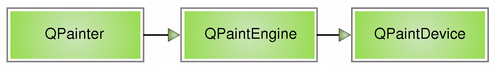
\includegraphics[width=\textwidth,height=!]{img/paintsystem-core.png}
  \caption{Schemat budowy systemu renderowania w bibliotece \emph{Qt}}
  \label{paintsystem-core}
\end{figure}

\section{GTK Broadway}
GTK Broadway jest młodym projektem powstałym w 2011 roku stworzonym przez Alexandra Larssona. Projekt nie posiada pełnej dokumentacji, dostępne są jedynie krótkie wpisy na blogu\cite{broadway1,broadway2}.

Broadway podobnie jak opisywana praca pozwala na uruchomienie aplikacji \emph{Gtk+} w przeglądarce. Broadway odwzorowuje każde okno aplikacji na jeden element \emph{canvas}. Zawartość okna jest aktualizowana poprzez komendy pobierane za pomocą żądania XHR (XMLHttpRequest) emulując w ten sposób HTTP pushing. Dodatkowo komendy są kompresowane przy pomocy algorytmu gzipem. Dane z wejścia przeglądarki są zbierane poprzez zdarzenia modelu DOM i wysyłane na serwer za pomocą WebSocketu. Dane o zawartości okien są przesyłane jako kopie regionów i kopie różnicowe, zaś obrazy jako data-URI zawierające obrazy PNG (zakodowane w base64). Jest to główna różnica między projektami -- w opisywanym projekcie dane przesyłane są w całkowicie inny sposób, szczegółowo opisany w kolejnych rozdziałach.

Backend ten nie jest domyślnie włączony w żadnej dużej dystrybucji systemu Linux i jego instalacja nie jest prosta. Wymaga ręcznej kompilacji całego pakietu Gtk+ z odpowiednimi flagami. Jest to bardzo kłopotliwe, gdyż wymaga to instalacji wielu zależności.

\chapter{Określenie problemu i proponowane rozwiązanie}
Przedmiotem pracy jest stworzenie prototypowego serwera oraz klienta HTML5. Zadaniem serwera jest jest udostępnienie usługi uruchamiającej aplikacje oparte o biblioteki \emph{Qt} i KDE. Zdalny dostęp do aplikacji uruchomionej w środowisku serwera jest dostępny poprzez interfejs HTML5 udostępniany przez instancję serwera.

Użytkownik serwisu w celu skorzystania z aplikacji \emph{Qt} zainstalowanej na serwerze wchodzi na odpowiedni adres przy użyciu nowoczesnej przeglądarki internetowej. Następnie wybiera interesujący go program i przejmuje nad nim kontrolę. Jest w stanie wyświetlić program w przeglądarce, który wizualnie odpowiada rzeczywistej instancji uruchomionej na serwerze. Wszystkie akcje myszy oraz klawiatury przechwycone przez przeglądarke są wysyłane do serwera, dzięki czemu użytkownik ma pełną kontrolę nad uruchomioną aplikacją. Należy również zaimplementować odpowiednik menedżera okien (ang. window manager) po stronie klienta, aby udostępnić użytkownikowi funkcjonalność pracy z wieloma oknami --- przesuwanie, rozszerzanie, zamykanie, oraz opcjonalnie minimalizowanie oraz maksymalizowanie.

// TODO: Wymagania (ogólne)
// TODO: Przypadki użycia
// TODO: Zachowanie systemu / software'u
// TODO: Struktura systemu / software'u

Postawione zadanie w głównej mierze polega na rozwiązaniu czterech podstawowych problemów:
\begin{enumerate}
  \item komunikacja między klientem a serwerem,
  \item komunikacja między klientem a aplikacją,
  \item uzyskanie informacji o wyglądzie elementów graficznego interfejsu aplikacji,
  \item symulacja interakcji użytkownika z interfejsem aplikacji.
\end{enumerate}

Na rysunku \ref{fig:arch} przedstawiono ideowy schemat architektury systemu rozwiązującego powyższe kwestie. 
Podstawą projektu jest jego modułowość, która separuje logikę odpowiedzialną za udostępnianie interfejsu WWW inicjującego proces aplikacji Qt od części stanowiącej węzeł komunikacyjny pomiędzy klientem a aplikacją Qt działąjącą po stronie serwera.
Można również zauważyć bardzo wyraźne rozgraniczenie między dwoma kanałami przesyłu danych, które wynika z konieczności umożliwienia korzystania z serwera wielu klientom. 
W dalszej części przedstawiono opis rozwiązań kolejnych problemów wraz z odniesieniem do odpowiednich części architektury na większym poziomie szczegółowości.

\begin{figure}
\centering
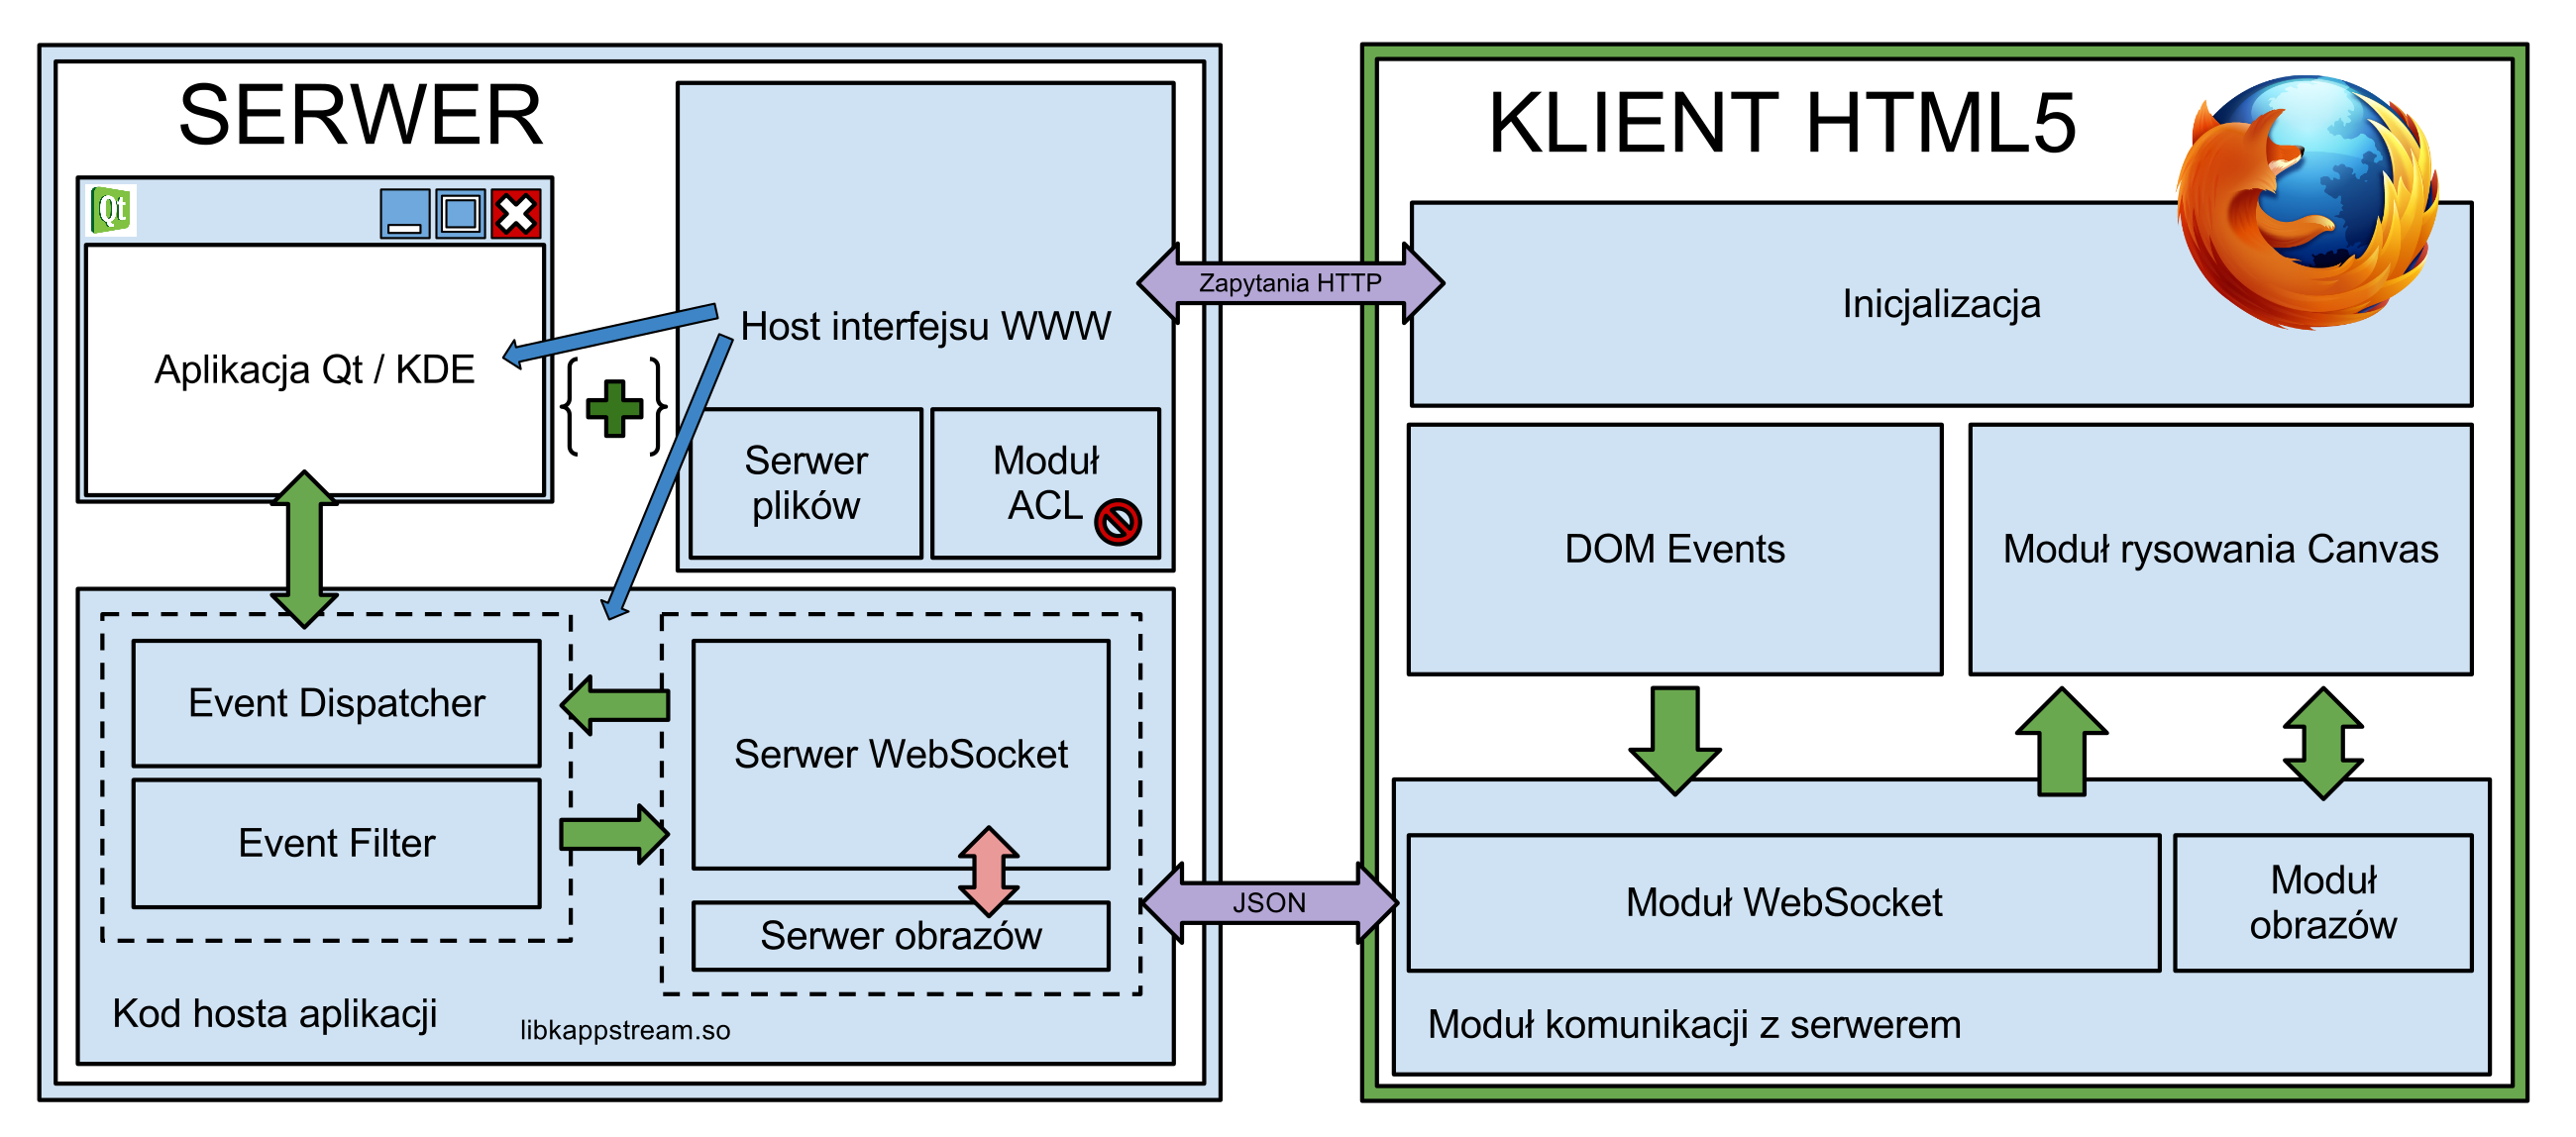
\includegraphics[width=1.0\linewidth]{img/arch}
\caption{Schemat architektury systemu.}
\label{fig:arch}
\end{figure}

\section{Komunikacja między klientem a serwerem}
%Specyfiką problemu jest jego dwuetapowość. W pierwszym etapipe klient inicjuje połączenie jednorazowo wysyłając zapytanie zawierające informacje o aplikacji, którą klient chce uruchomić oraz identyfikatorze klienta. W drugiej kolejności wymagane jest utworzenie kanału komunikacyjnego między klientem a procesem aplikacji. 

Do realizacji tego zadania stworzony został prosty serwer WWW działający w oparciu o protokół \emph{HTTP}. Jego architektura została przedstawiona na rysunku \ref{fig:arch-www}. Jako zasób domyślny udostępnia on listę dostępnych aplikacji, które klient może uruchomić. Lista ta jest w pełni konfigurowalna po stronie serwera. Inicjalizacja połączenia polega na wysłaniu przez klienta identyfikatora wybranej aplikacji. Serwer po pomyślnej weryfikacji przydziela klientowi unikatowy identyfikator sesji, uruchamia proces aplikacji i wysyła klientowi skrypt w języku JavaScript zajmujący się przetwarzaniem po stronie klienta. Każde zapytanie klienta jest weryfikowane za pomocą modułu ACL\footnote{ang. Access Control List}, który sprawdza czy konfiguracja serwera zezwala na uruchamianie żądanych aplikacji. Szczegółowy opis modułu przedstawiono w sekcji \ref{sec:server-security}.

\begin{figure}[H]
\centering
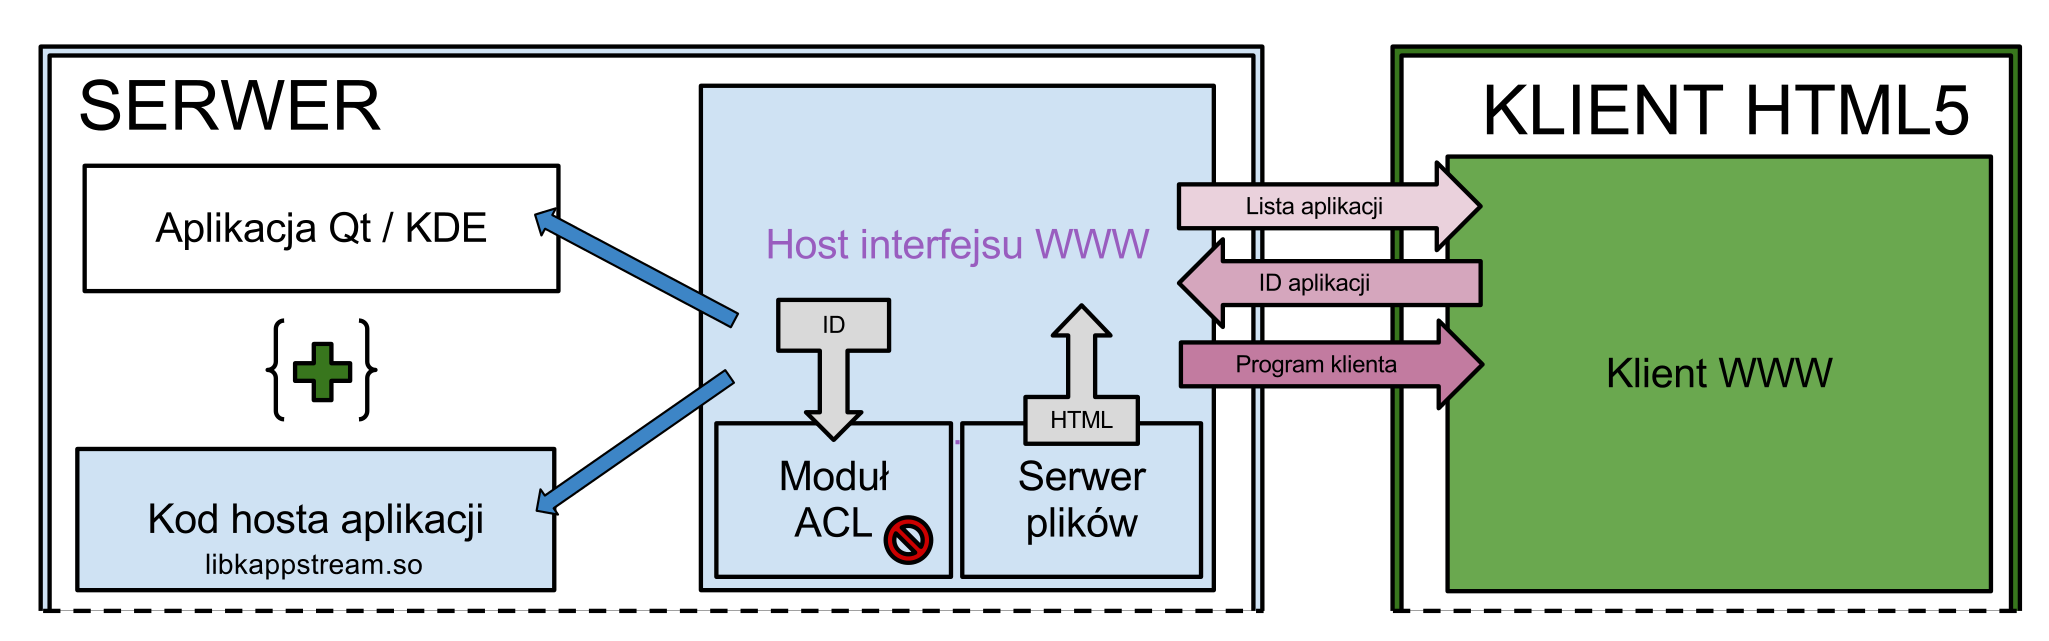
\includegraphics[width=1.0\linewidth]{img/arch-www}
\caption{Schemat komunikacji z serwerem WWW.}
\label{fig:arch-www}
\end{figure}

\section{Komunikacja między klientem a aplikacją}

// TODO: Opis do cz. teoretycznej (pogrubione)

Do rozwiązania tego problemu konieczne jest utworzenie ciągłego kanału komunikacyjnego między klientem a procesem aplikacji, za pomocą którego będzie możliwe przesyłanie informacji o wyglądzie interfejsu aplikacji oraz informowanie aplikacji o zdarzeniach generowanych przez użytkownika po stronie przeglądarki. Jako, że za cel przyjęte zostało założenie o nieingerowaniu bezpośrednio w kod skompilowanych już aplikacji, postawiono na technikę umożliwiającą załadowanie kodu biblioteki dynamicznej do przestrzeni pamięciowej procesu aplikacji tuż przed jego uruchomieniem. Kod ten ma za zadanie utrzymanie połączenia oraz transmisję danych między klientem a aplikacją.

\begin{figure}[H]
\centering
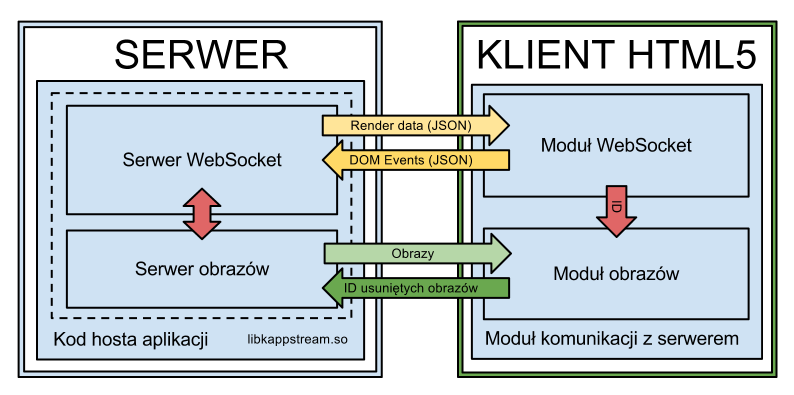
\includegraphics[width=1.0\linewidth]{img/arch-socket}
\caption{Schemat komunikacji z modułem WebSocket.}
\label{fig:arch-socket}
\end{figure}

\section{Uzyskanie informacji o wyglądzie elementów graficznego interfejsu aplikacji}
Każdy element graficznego interfejsu aplikacji (QWidget) jest renderowany w momencie odebrania zdarzenia QPaintEvent z kolejki zdarzeń głównego wątku aplikacji. Dzięki temu istnieje łatwy sposób na uzyskanie informacji o tym kiedy oraz ktory element należy przerenderować aby uaktualnić jego wygląd po stronie klienta. Problemem w dalszyb ciągu pozostaje jednak sposób na uzyskanie informacji o samym wyglądzie. 

Proponowane rozwiązanie polega na zaimplementowaniu abstrakcyjnego urządzenia wyjściowego reprezentującego przeglądarkę WWW po stronie klienta (patrz podrozdział \ref{system_rysowania}). Odpowiednio implementując klasy \emph{QPaintEngine} oraz \emph{QPaintDevice} możliwe staje się uzyskanie szczegółowych informacji dotyczących wygądu widgetów co z kolei umozliwia stworzenie \bf{innowacyjnego} formatu przesyłanych danych. Zamiast przesyłać bitmapy z wyrenderowanym elementem można wysłać informację o kolorach, punktach, liniach i innych podstawowych elementach, które zostaną narysowane na urządzeniu docelowym jakim po stronie klienta jest przeglądarka WWW z obsługą elementów \emph{canvas}.


// TODO Komentarz Co to znaczy innowacyjnego?

\section{Symulacja interakcji użytkownika z interfejsem aplikacji}
Interakcja użytkownika z aplikacją sprowadza się do obsługi następujących zdarzeń:
\begin{enumerate}
  \item ruch myszy nad elementem,
  \item wciśnięcie, zwolnienie oraz dwuklik przycisku myszy,
  \item zmiana położenia kółka myszy,
  \item wciśnięcie oraz zwolnienie klawiszy na klawiaturze,
  \item zmiana rozmiaru okna aplikacji poprzez przeciąganie jego krawędzi,
  \item zamknięcie, minimalizacja lub maksymalizacja okna aplikacji.
\end{enumerate}
Większość z wyżej wymienionych elementów jest obsługiwana jako zdarzenia w języku JavaScript większości dzisiejszych przeglądarek. Proponowane podejście na rozwiązanie tego zagadnienia polega na stworzeniu formatu danych bazując na notacji JSON (JavaScript Object Notation). Dane w tym formacie przesyłane do serwera są następnie poddawane walidacji i konwersji na obiekty zdarzeń biblioteki \emph{Qt}. Zdarzenia takie są następnie przesyłane do kolejki zdarzeń w głównym wątku aplikacji.

Odbiorcą zdarzenia jest obiekt, który na rysunku \ref{fig:arch-hook} został oznaczony jako Event Dispather. Moduł ten jest następnie odpowiedzialny za podjęcie akcji w odpowiedzi na dane zdarzenie, polegających na wywołaniu odpowiednich metod na elemencie interfejsu graficznego aplikacji, który wygenerował dane zdarzenie po stronie przeglądarki bazując na hierarchicznej budowie interfejsu użytkownika.
Wyjątkami są tutaj zdarzenia klawiatury, które nie mają bezpośredniego odbiorcy w momencie ich zaistnienia. Aplikacja na ogół sama decyduje o tym, który element powinien odebrać zdarzenie. Domyślnie jest to widget, który atualnie posiada tzw. focus, a to z kolei zależy od poprzednich zdarzeń oraz logiki samego programu. W celu symulacji podobnego zachowania moduł Event Dispather wybiera element interfejsu bazując na aktualnym stanie aplikacji i wysyła informację o wciśnięciu wirtualnych klawiszy. 

Taka struktura modułu obsługi zdarzeń zapewnia jednolitość działania aplikacji pomiędzy różnymi wersjami biblioteki Qt.

\section{Odtwarzanie aplikacji po stronie klienta}
Aby umożliwić renderowanie elementów po stronie klienta należało utworzyć wspólny format danych bazując na wejściu ze strony biblioteki Qt oraz potrzebnych danych wyjściowych dla obiektu Canvas w języku HTML5. 

Każda komenda rysowania po stronie klienta składa się z podstawowych informacji dotyczących rysowanego obiektu, takich jak: identyfikator, pozycja czy rozmiar, oraz listy prostych elementów z których danych obiekt jest złożony (linie, prostokąty, etc.). Poniżej przedstawiono format pojedyńczej komendy rysowania.


\begin{lstlisting}[language=JavaScript,caption=Komenda renderowania elementu interfejsu]
{
  "command":"draw",
  "widget":{
    "id": 12431,          // Identyfikator
    ["z": 0,]             // Pozycja na stosie obiektow potomnych
    "name":"QLineEdit",   // Nazwa obiektu
    "flags": 0x1029,      // Flagi obiektu (definiuja jego typ 
                          // i wlasciwosci)
    "x": 100,             // Pozycja X
    "y": 120,             // Pozycja Y
    "w": 200,             // Szerokosc
    "h": 150,             // Wysokosc
    "r":{                 // Renderowany obszar elementu
      "x": 0,             // Pozycja obszaru X
      "y": 0,             // Pozycja obszaru Y
      "w": 200,           // Szerokosc obszaru
      "h": 150,           // Wysokosc obszaru
    }
  },
  "render":[]             // Lista elementow do narysowania
}
\end{lstlisting}

Poniżej w kolejności alfabetycznej przedstawiono elementy, z których może być zbudowany każdy obiekt klasy QWidget. Każdy opis zawiera deklarację metody podklasy QPaintEngine wykorzystywanej po stronie serwera, format przesyłanych danych oraz sposób interpretacji tych danych po stronie klienta.

\subsection{Elipsy}
\begin{lstlisting}[language=C++,numbers=none]
virtual void QPaintEngine::drawEllipse( const QRectF & rect );
virtual void QPaintEngine::drawEllipse( const QRect & rect );
\end{lstlisting}
\begin{lstlisting}[language=JavaScript,numbers=none]
{
  "t":"ellipse",
  "x":0.0,       // Pozycja srodka X
  "y":0.0,       // Pozycja srodka Y
  "w":10.0,      // Srednica pozioma
  "h":10.0       // Srednica pionowa
}
\end{lstlisting}

\subsection{Kwadraty}
\begin{lstlisting}[language=C++,numbers=none]
virtual void QPaintEngine::drawRects( const QRectF * rects, 
                                      int rectCount );
virtual void QPaintEngine::drawRects( const QRect * rects, 
                                      int rectCount );
\end{lstlisting}
\begin{lstlisting}[language=JavaScript,numbers=none]
{
  "t":"rect",
  "x":0.0,      // Pozycja lewego-gornego wierzcholka X
  "y":0.0,      // Pozycja lewego-gornego wierzcholka Y
  "w":10.0,     // Szerokosc
  "h":10.0      // Wysokosc
}
\end{lstlisting}

\subsection{Linie}
\begin{lstlisting}[language=C++,numbers=none]
virtual void QPaintEngine::drawLines( const QLineF * lines, 
                                      int lineCount );
virtual void QPaintEngine::drawLines( const QLine * lines, 
                                      int lineCount );
\end{lstlisting}
\begin{lstlisting}[language=JavaScript,numbers=none]
{
  "t":"line",
  "xs":0.0,    // Pozycja startowa X
  "ys":0.0,    // Pozycja startowa Y
  "xe":10.0,   // Pozycja koncowa X
  "ye":10.0    // Pozycja koncowa Y
}
\end{lstlisting}

\subsection{Obrazy}
\begin{lstlisting}[language=C++,numbers=none]
virtual void QPaintEngine::drawImage( const QRectF & rectangle, 
                                      const QImage & image, 
                                      const QRectF & sr, 
                                      Qt::ImageConversionFlags flags = Qt::AutoColor );
virtual void QPaintEngine::drawPixmap( const QRectF & r, 
                                       const QPixmap & pm, 
                                       const QRectF & sr );
virtual void QPaintEngine::drawTiledPixmap( const QRectF & rect, 
                                            const QPixmap & pixmap, 
                                            const QPointF & p );
\end{lstlisting}
\begin{lstlisting}[language=JavaScript,numbers=none]
{
  "t":"image",
  "data":"Ja8SA9c72b71HDj8", // Identyfikator obrazu
  "x":0.0,                   // Pozycja X
  "y":0.0                    // Pozycja Y
}
\end{lstlisting}

Pełna implementacja, natywnie wspierane w \emph{canvas} za pomocą metody drawImage.

\subsection{Wielokąty}
\begin{lstlisting}[language=C++,numbers=none]
virtual void QPaintEngine::drawPolygon( const QPointF * points, 
                                        int pointCount, 
                                        PolygonDrawMode mode );
virtual void QPaintEngine::drawPolygon( const QPoint * points, 
                                        int pointCount, 
                                        PolygonDrawMode mode );
\end{lstlisting}
\begin{lstlisting}[language=JavaScript,numbers=none]
{
  "t":"polygon",
  "mode":0, // 0: QPaintEngine::OddEvenMode
            // 1: QPaintEngine::WindingMode
            // 2: QPaintEngine::ConvexMode
            // 3: QPaintEngine::PolylineMode	
            // http://doc.qt.digia.com/stable/qpaintengine.html#PolygonDrawMode-enum
  "data":   // Lista punktow do polaczenia
    [
      [0.0,0.0],
      [10.0,10.0],
      [123.0,123.0]
    ]
}
\end{lstlisting}

Pełna implementacja, natywnie wspierane w \emph{canvas} za pomocą metod \emph{moveTo}, \emph{lineTo} oraz \emph{closePath}.

\subsection{Punkty}

\begin{lstlisting}[language=C++,numbers=none]
virtual void QPaintEngine::drawPoints( const QPointF * points, 
                                       int pointCount );
virtual void QPaintEngine::drawPoints( const QPoint * points, 
                                       int pointCount );
\end{lstlisting}
\begin{lstlisting}[language=JavaScript,numbers=none]
{
  "t":"points",
  "data":              // Lista punktow
    [
      [0.0,0.0],
      [10.0,10.0],
      [123.0,123.0]
    ]
},
\end{lstlisting}

Pełna implementacja, natywnie wspierane w \emph{canvas}, za pomocą \emph{strokeRect} rysowany jest kwadrat o rozmiarach 1 na 1 piksel.

\subsection{Ścieżki}
\begin{lstlisting}[language=C++,numbers=none]
virtual void QPaintEngine::drawPath( const QPainterPath & path );
\end{lstlisting}
\begin{lstlisting}[language=JavaScript,numbers=none]
{
  "t":"path",
  "data":          // Lista punktow
    [
      ["t":0,"p":[[0,0]]],      // moveTo
      ["t":1,"p":[[10,10]]],    // lineTo
      ["t":2,"p":[[10,10],[100,100]]],  // quadTo
      ["t":2,"p":[[10,10],[100,100],[1000,1000]]],  // cubicTo
    ],
  "fill":0 // 0: Qt::OddEvenFill
           // 1: Qt::WindingFill
           // http://doc.qt.digia.com/stable/qt.html#FillRule-enum
}
\end{lstlisting}

Pełna implementacja, natywnie wspierane w \emph{canvas} za pomocą metod \emph{lineTo}, \emph{lineTo}, \emph{quadraticCurveTo} oraz \emph{bezierCurveTo}.

\subsection{Tekst}
\begin{lstlisting}[language=C++,numbers=none]
virtual void QPaintEngine::drawTextItem( const QPointF & p, 
                                         const QTextItem & textItem );
\end{lstlisting}
\begin{lstlisting}[language=JavaScript,numbers=none]
{
  "t":"text",
  "data":
  {
    "text":"Przykladowy tekst",     // Tekst w kodowaniu UTF8
    "ascent":0,                     // Dystans od linii bazowej do 
                                    // najwyzej polozonego punktu
    "descent":0,                    // Dystans od linii bazowej do 
                                    // najnizej polozonego punktu
    "x":0,                          // Pozycja X
    "y":0,                          // Pozycja Y
    "font":"CSS-format font string" // Informacje o czcionce 
                                    // w formacie CSS
  }
}
\end{lstlisting}

\section{Wewnętrzne przepływy danych w module WebSocket serwera}
Moduł serwera służący do przesyłu danych między aplikacją a klientem złożony jest z dwóch głównych części:
\begin{enumerate}
\item komunikacji z aplikacją,
\item komunikacji z klientem.
\end{enumerate}
Komunikują się one przesyłając dane w formacie JSON. Event Dispather posiada jedno wejście przyjmujące opis zdarzeń zaistniałych po stronie klienta. Event Filter posiada dwa wyjścia, którymi przekazuje dane do serwera WebSocket, który następnie przekazuje je klientowi. Jedno wyjście przekazuje opis graficznych elementów interfejsu. Drugie natomiast obrazy w formacie PNG. Powód dla którego postanowiono oddzielić przesyłąnie obrazów od przesyłania opisu w formasie JSON jest zbyt duży narzut na rozmiar pliku graficznego po konwersji do postaci tekstowej. Serwer WebSocket nie wysyła więc obrazów bezpośrednio do klienta. Przesyła mu jedynie indentyfikator obrazu a same dane są przekazywane do serwera obrazów, który stanowi bufor dla plików graficznych. Bufor ten jest na bieżąco opróżniany w momencie gdy klient zdecyduje się pobrać dany obraz.

\begin{figure}[H]
\centering
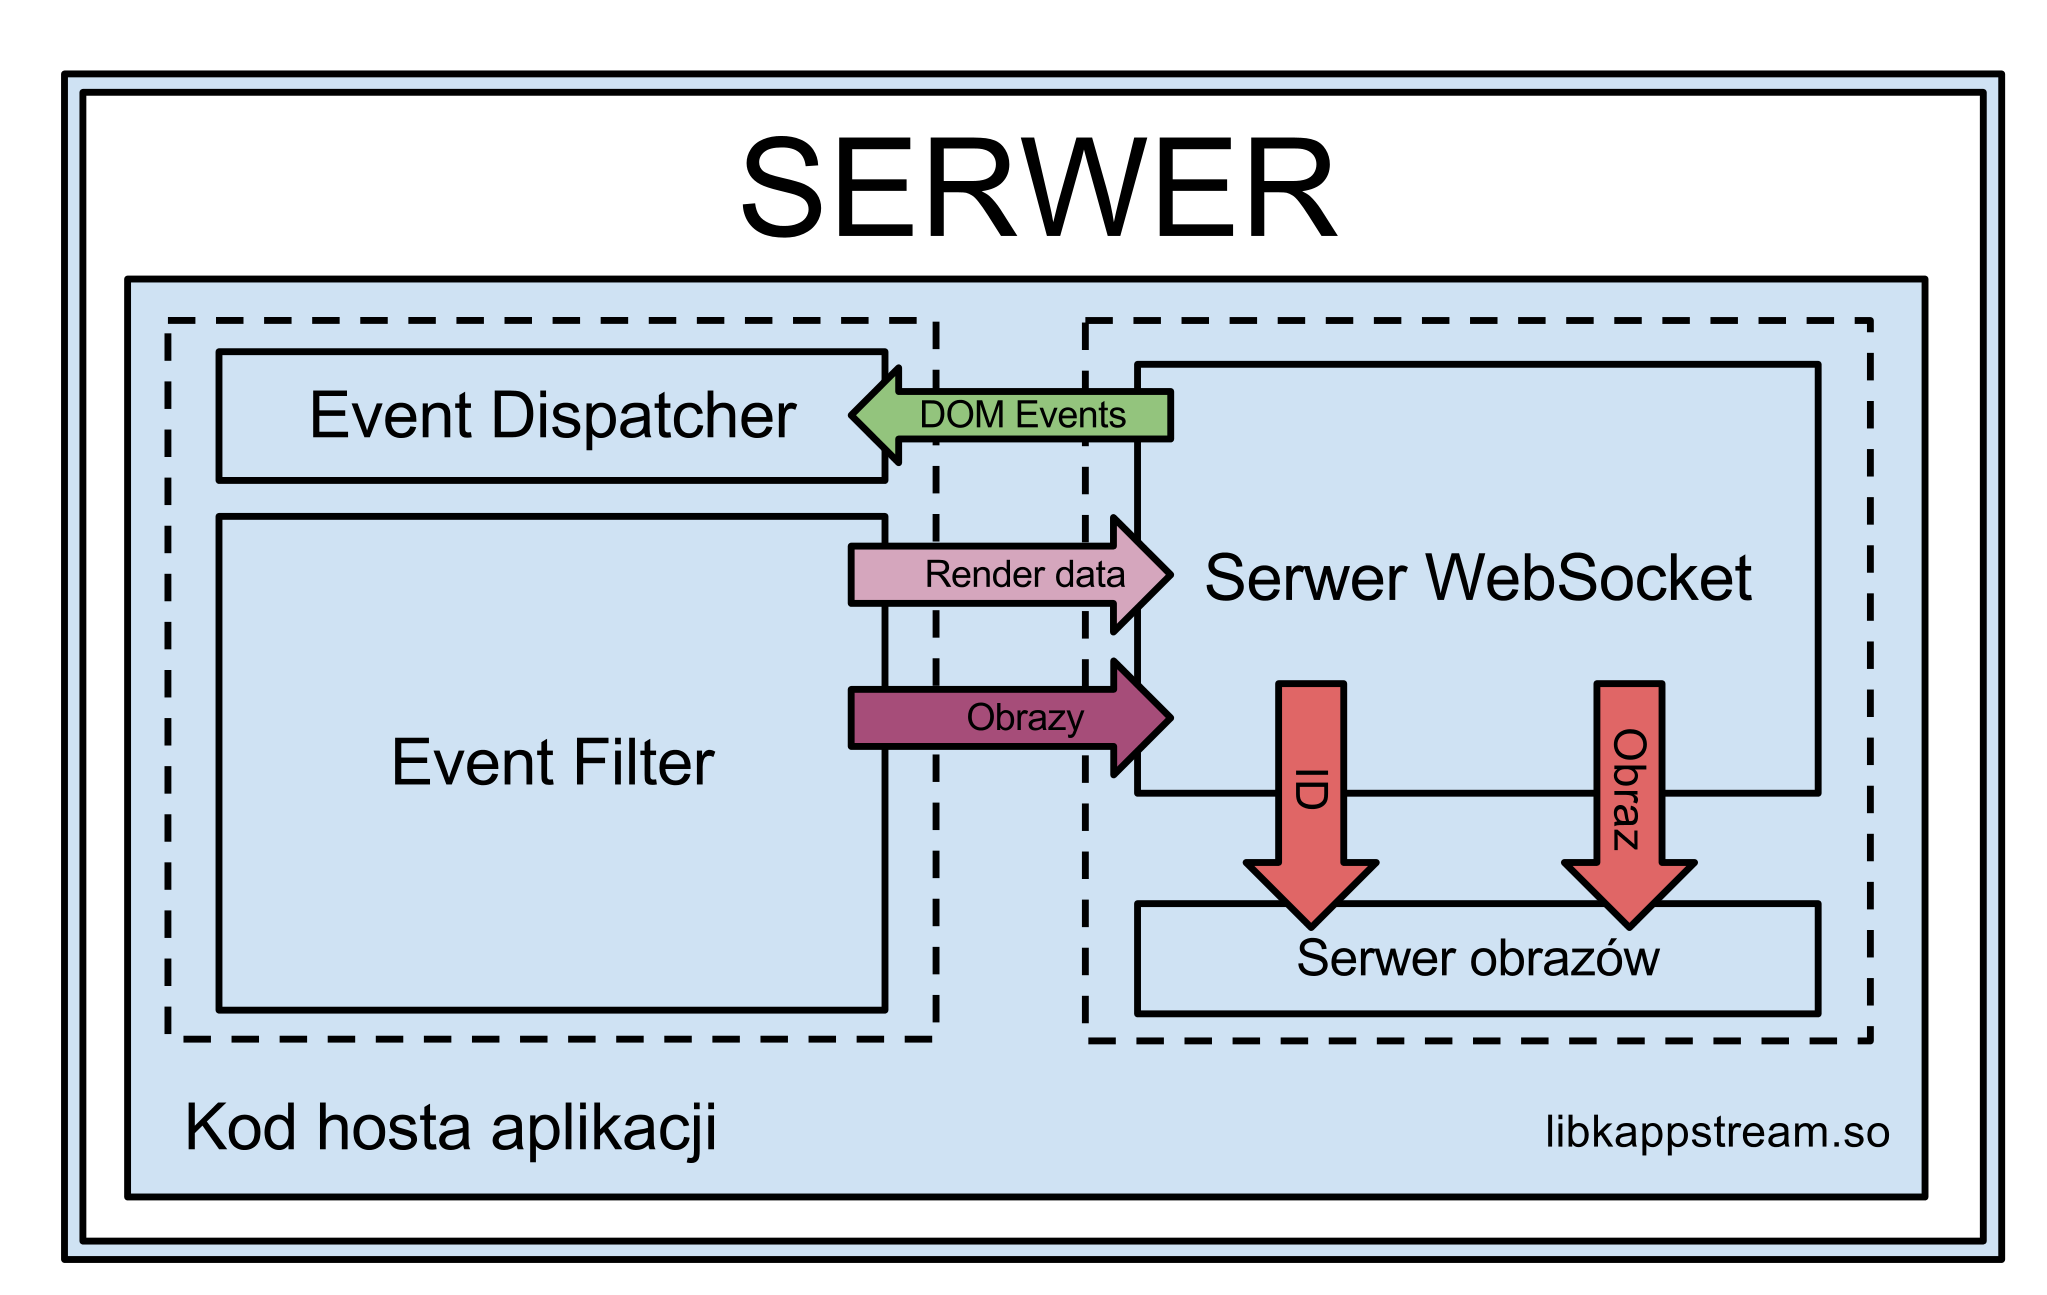
\includegraphics[width=0.8\linewidth]{img/arch-lib}
\caption{Schemat wewnętrznych przepływów danych w module WebSocket.}
\label{fig:arch-lib}
\end{figure}


\section{Zabezpieczenie serwera}
Ponieważ jednym z celów projektu było umożliwienie uruchamiania pełnoprawnych aplikacji zainstalowanych na systemie operacyjnym serwera, kluczową staje się możliwość blokowania nieautoryzowanego dostępu do wrażliwych lub potencjalnie niebezpiecznych aplikacji.

W związku z powyższym, stworzono mechanizm list \emph{ACL} (ang. Access Control Lists), który pozwala administratorowi systemu na zdefiniowane, które aplikacje mogą być uruchamiane przez klientów, a w przypadku których zostanie wyświetlony komunikatu o braku dostępu.

Listy kontroli dostępu przechowywane są w pliku konfiguracyjnym serwera w postaci danych w formacie \emph{XML}\footnote{(ang. Extensible Markup Language}. Nazwy aplikacji w postaci komend linii poleceń mogą więc być definiowane ręcznie w dowolnym edytorze tekstowym lub za pomocą pliku wykonywalnego serwera poprzez poniższe argumentów wywołania programu:

\begin{itemize}
\item \emph{accept-all}
spowoduje zniesienie wszystkich wcześniej wprowadzonych obostrzeń i możliwe będzie uruchomienie wszystkich aplikacji zainstalowanych na serwerze,
\item \emph{reject-all}
spowoduje zablokowanie wszystkich zapytań serwera. Komenda ta powinna stanowić pierwszy krok w etapie budowy list dostępu,
\item \emph{accept nazwa-aplikacji} \footnote{Nazwa aplikacji oznacza pełną komendę wiersza poleceń (wraz z możliwymi argumentami), która spowoduje uruchomienie aplikacji. Może to być również ścieżka bezwzględna do pliku wykonywalnego aplikacji.}
spowoduje, że aplikacja o podanej nazwie będzie mogła być uruchamiana przez serwer,
\item \emph{reject nazwa-aplikacji},
komenda blokujaca możliwość uruchamiania aplikacji o podanej nazwie.
\end{itemize}

Serwer, ze względów bezpieczeństwa, od razu po zainstalowaniu domyslnie blokuje wszystkie zapytania klientów i oczekuje się od administratora serwera skonfigurowania list \emph{ACL} według uznania. Zmiana ustawień serwera wymaga jego ponownego uruchomienia.

\section{Komunikacja między klientem a serwerem}
%Specyfiką problemu jest jego dwuetapowość. W pierwszym etapipe klient inicjuje połączenie jednorazowo wysyłając zapytanie zawierające informacje o aplikacji, którą klient chce uruchomić oraz identyfikatorze klienta. W drugiej kolejności wymagane jest utworzenie kanału komunikacyjnego między klientem a procesem aplikacji. 

Do realizacji tego zadania stworzony został prosty serwer WWW działający w oparciu o protokół \emph{HTTP}. Jego architektura została przedstawiona na rysunku \ref{fig:arch-www}. Jako zasób domyślny udostępnia on listę dostępnych aplikacji, które klient może uruchomić. Lista ta jest w pełni konfigurowalna po stronie serwera. Inicjalizacja połączenia polega na wysłaniu przez klienta identyfikatora wybranej aplikacji. Serwer po pomyślnej weryfikacji przydziela klientowi unikatowy identyfikator sesji, uruchamia proces aplikacji i wysyła klientowi skrypt w języku JavaScript zajmujący się przetwarzaniem po stronie klienta. Każde zapytanie klienta jest weryfikowane za pomocą modułu ACL\footnote{ang. Access Control List}, który sprawdza czy konfiguracja serwera zezwala na uruchamianie żądanych aplikacji. Szczegółowy opis modułu przedstawiono w sekcji \ref{sec:server-security}.

\begin{figure}[H]
\centering
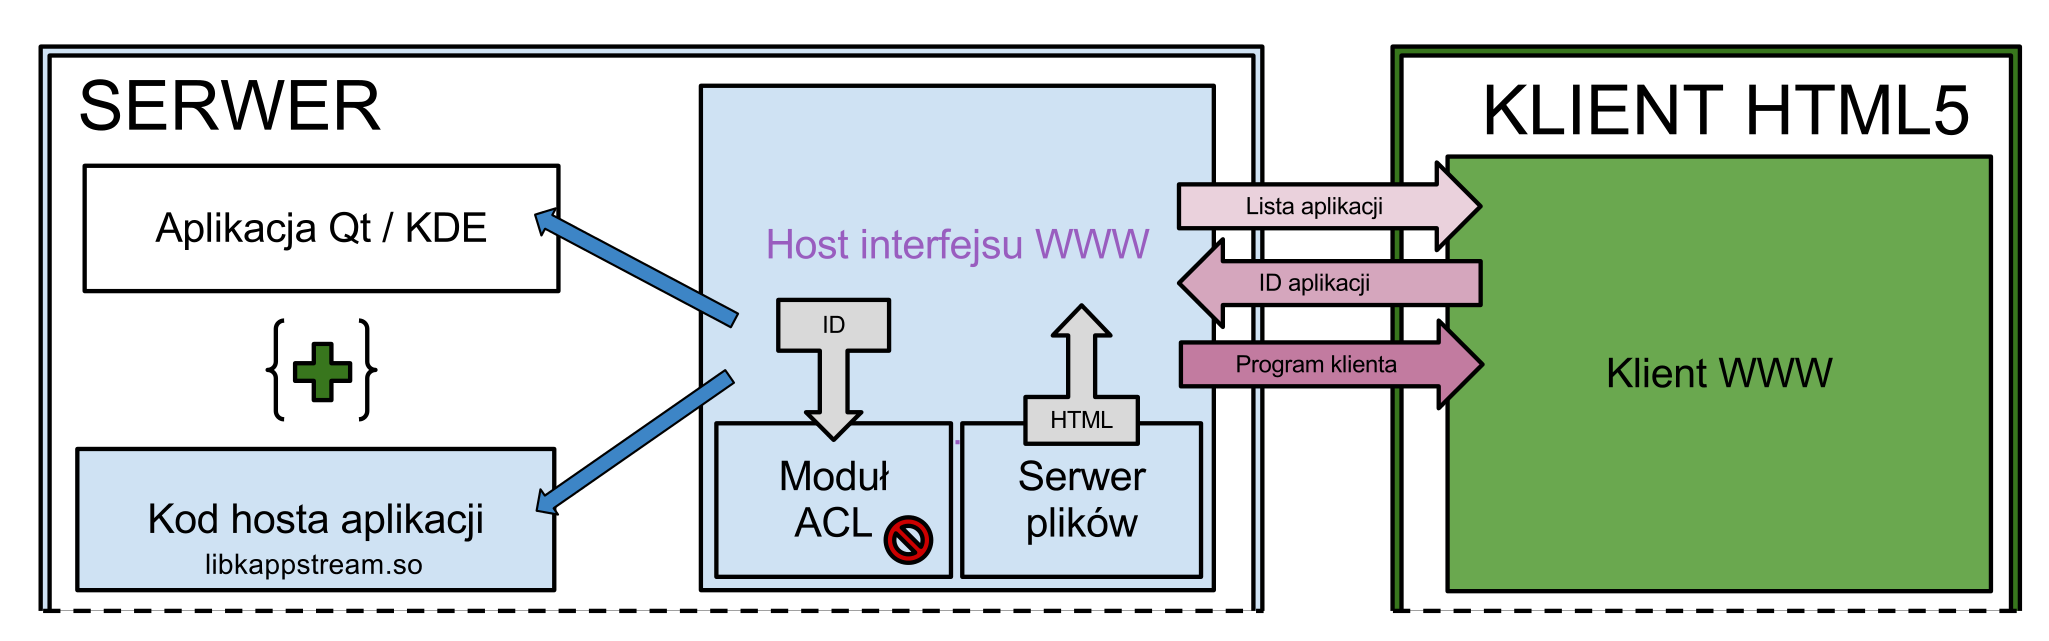
\includegraphics[width=1.0\linewidth]{img/arch-www}
\caption{Schemat komunikacji z serwerem WWW.}
\label{fig:arch-www}
\end{figure}

\section{Komunikacja między klientem a aplikacją}

// TODO: Opis do cz. teoretycznej (pogrubione)

Do rozwiązania tego problemu konieczne jest utworzenie ciągłego kanału komunikacyjnego między klientem a procesem aplikacji, za pomocą którego będzie możliwe przesyłanie informacji o wyglądzie interfejsu aplikacji oraz informowanie aplikacji o zdarzeniach generowanych przez użytkownika po stronie przeglądarki. Jako, że za cel przyjęte zostało założenie o nieingerowaniu bezpośrednio w kod skompilowanych już aplikacji, postawiono na technikę umożliwiającą załadowanie kodu biblioteki dynamicznej do przestrzeni pamięciowej procesu aplikacji tuż przed jego uruchomieniem. Kod ten ma za zadanie utrzymanie połączenia oraz transmisję danych między klientem a aplikacją.

\begin{figure}[H]
\centering
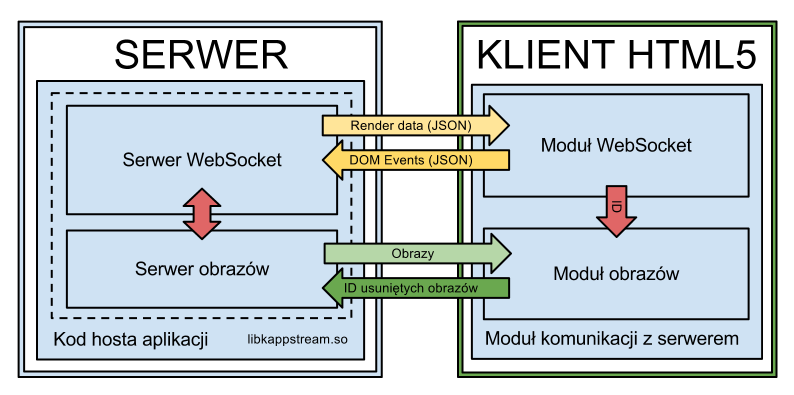
\includegraphics[width=1.0\linewidth]{img/arch-socket}
\caption{Schemat komunikacji z modułem WebSocket.}
\label{fig:arch-socket}
\end{figure}

\section{Uzyskanie informacji o wyglądzie elementów graficznego interfejsu aplikacji}

Każdy element graficznego interfejsu aplikacji (QWidget) jest renderowany w momencie odebrania zdarzenia QPaintEvent z kolejki zdarzeń głównego wątku aplikacji. Dzięki temu istnieje łatwy sposób na uzyskanie informacji o tym kiedy oraz ktory element należy przerenderować aby uaktualnić jego wygląd po stronie klienta. Problemem w dalszyb ciągu pozostaje jednak sposób na uzyskanie informacji o samym wyglądzie. 

Proponowane rozwiązanie polega na zaimplementowaniu abstrakcyjnego urządzenia wyjściowego reprezentującego przeglądarkę WWW po stronie klienta (patrz podrozdział \ref{system_rysowania}). Odpowiednio implementując klasy \emph{QPaintEngine} oraz \emph{QPaintDevice} możliwe staje się uzyskanie szczegółowych informacji dotyczących wygądu widgetów co z kolei umozliwia stworzenie \bf{innowacyjnego} formatu przesyłanych danych. Zamiast przesyłać bitmapy z wyrenderowanym elementem można wysłać informację o kolorach, punktach, liniach i innych podstawowych elementach, które zostaną narysowane na urządzeniu docelowym jakim po stronie klienta jest przeglądarka WWW z obsługą elementów \emph{canvas}.


// TODO Komentarz Co to znaczy innowacyjnego?

\section{Symulacja interakcji użytkownika z interfejsem aplikacji}
Interakcja użytkownika z aplikacją sprowadza się do obsługi następujących zdarzeń:
\begin{enumerate}
  \item ruch myszy nad elementem,
  \item wciśnięcie, zwolnienie oraz dwuklik przycisku myszy,
  \item zmiana położenia kółka myszy,
  \item wciśnięcie oraz zwolnienie klawiszy na klawiaturze,
  \item zmiana rozmiaru okna aplikacji poprzez przeciąganie jego krawędzi,
  \item zamknięcie, minimalizacja lub maksymalizacja okna aplikacji.
\end{enumerate}
Większość z wyżej wymienionych elementów jest obsługiwana jako zdarzenia w języku JavaScript większości dzisiejszych przeglądarek. Proponowane podejście na rozwiązanie tego zagadnienia polega na stworzeniu formatu danych bazując na notacji JSON (JavaScript Object Notation). Dane w tym formacie przesyłane do serwera są następnie poddawane walidacji i konwersji na obiekty zdarzeń biblioteki \emph{Qt}. Zdarzenia takie są następnie przesyłane do kolejki zdarzeń w głównym wątku aplikacji.

Odbiorcą zdarzenia jest obiekt, który na rysunku \ref{fig:arch-hook} został oznaczony jako Event Dispather. Moduł ten jest następnie odpowiedzialny za podjęcie akcji w odpowiedzi na dane zdarzenie, polegających na wywołaniu odpowiednich metod na elemencie interfejsu graficznego aplikacji, który wygenerował dane zdarzenie po stronie przeglądarki bazując na hierarchicznej budowie interfejsu użytkownika.
Wyjątkami są tutaj zdarzenia klawiatury, które nie mają bezpośredniego odbiorcy w momencie ich zaistnienia. Aplikacja na ogół sama decyduje o tym, który element powinien odebrać zdarzenie. Domyślnie jest to widget, który atualnie posiada tzw. focus, a to z kolei zależy od poprzednich zdarzeń oraz logiki samego programu. W celu symulacji podobnego zachowania moduł Event Dispather wybiera element interfejsu bazując na aktualnym stanie aplikacji i wysyła informację o wciśnięciu wirtualnych klawiszy. 

Taka struktura modułu obsługi zdarzeń zapewnia jednolitość działania aplikacji pomiędzy różnymi wersjami biblioteki Qt.

\section{Zabezpieczenie aplikacji}
Ponieważ jednym z celów projektu było umożliwienie uruchamiania pełnoprawnych aplikacji zainstalowanych na systemie operacyjnym serwera, kluczową staje się możliwość blokowania nieautoryzowanego dostępu do wrażliwych lub potencjalnie niebezpiecznych aplikacji.

W związku z powyższym, stworzono mechanizm list \emph{ACL} (ang. Access Control Lists), który pozwala administratorowi systemu na zdefiniowane, które aplikacje mogą być uruchamiane przez klientów, a w przypadku których zostanie wyświetlony komunikatu o braku dostępu.

Listy kontroli dostępu przechowywane są w pliku konfiguracyjnym serwera w postaci danych w formacie \emph{XML}\footnote{(ang. Extensible Markup Language}. Nazwy aplikacji w postaci komend linii poleceń mogą więc być definiowane ręcznie w dowolnym edytorze tekstowym lub za pomocą pliku wykonywalnego serwera poprzez poniższe argumentów wywołania programu:

\begin{itemize}
\item \emph{accept-all}
spowoduje zniesienie wszystkich wcześniej wprowadzonych obostrzeń i możliwe będzie uruchomienie wszystkich aplikacji zainstalowanych na serwerze,
\item \emph{reject-all}
spowoduje zablokowanie wszystkich zapytań serwera. Komenda ta powinna stanowić pierwszy krok w etapie budowy list dostępu,
\item \emph{accept nazwa-aplikacji} \footnote{Nazwa aplikacji oznacza pełną komendę wiersza poleceń (wraz z możliwymi argumentami), która spowoduje uruchomienie aplikacji. Może to być również ścieżka bezwzględna do pliku wykonywalnego aplikacji.}
spowoduje, że aplikacja o podanej nazwie będzie mogła być uruchamiana przez serwer,
\item \emph{reject nazwa-aplikacji},
komenda blokujaca możliwość uruchamiania aplikacji o podanej nazwie.
\end{itemize}

Serwer, ze względów bezpieczeństwa, od razu po zainstalowaniu domyslnie blokuje wszystkie zapytania klientów i oczekuje się od administratora serwera skonfigurowania list \emph{ACL} według uznania. Zmiana ustawień serwera wymaga jego ponownego uruchomienia.

\chapter{Implementacja}
\section{Renderowanie}
Aby umożliwić renderowanie elementów po stronie klienta należało utworzyć wspólny format danych bazując na wejściu ze strony biblioteki Qt oraz potrzebnych danych wyjściowych dla obiektu Canvas w języku HTML5. 

Każda komenda rysowania po stronie klienta składa się z podstawowych informacji dotyczących rysowanego obiektu, takich jak: identyfikator, pozycja czy rozmiar, oraz listy prostych elementów z których danych obiekt jest złożony (linie, prostokąty, etc.). Poniżej przedstawiono format pojedyńczej komendy rysowania.


\begin{lstlisting}[language=JavaScript,caption=Komenda renderowania elementu interfejsu]
{
  "command":"draw",
  "widget":{
    "id": 12431,          // Identyfikator
    ["z": 0,]             // Pozycja na stosie obiektow potomnych
    "name":"QLineEdit",   // Nazwa obiektu
    "flags": 0x1029,      // Flagi obiektu (definiuja jego typ 
                          // i wlasciwosci)
    "x": 100,             // Pozycja X
    "y": 120,             // Pozycja Y
    "w": 200,             // Szerokosc
    "h": 150,             // Wysokosc
    "r":{                 // Renderowany obszar elementu
      "x": 0,             // Pozycja obszaru X
      "y": 0,             // Pozycja obszaru Y
      "w": 200,           // Szerokosc obszaru
      "h": 150,           // Wysokosc obszaru
    }
  },
  "render":[]             // Lista elementow do narysowania
}
\end{lstlisting}

Poniżej w kolejności alfabetycznej przedstawiono elementy, z których może być zbudowany każdy obiekt klasy QWidget. Każdy opis zawiera deklarację metody podklasy QPaintEngine wykorzystywanej po stronie serwera, format przesyłanych danych oraz sposób interpretacji tych danych po stronie klienta.

\subsection{Elipsy}
\begin{lstlisting}[language=C++,numbers=none]
virtual void QPaintEngine::drawEllipse( const QRectF & rect );
virtual void QPaintEngine::drawEllipse( const QRect & rect );
\end{lstlisting}
\begin{lstlisting}[language=JavaScript,numbers=none]
{
  "t":"ellipse",
  "x":0.0,       // Pozycja srodka X
  "y":0.0,       // Pozycja srodka Y
  "w":10.0,      // Srednica pozioma
  "h":10.0       // Srednica pionowa
}
\end{lstlisting}

\subsection{Kwadraty}
\begin{lstlisting}[language=C++,numbers=none]
virtual void QPaintEngine::drawRects( const QRectF * rects, 
                                      int rectCount );
virtual void QPaintEngine::drawRects( const QRect * rects, 
                                      int rectCount );
\end{lstlisting}
\begin{lstlisting}[language=JavaScript,numbers=none]
{
  "t":"rect",
  "x":0.0,      // Pozycja lewego-gornego wierzcholka X
  "y":0.0,      // Pozycja lewego-gornego wierzcholka Y
  "w":10.0,     // Szerokosc
  "h":10.0      // Wysokosc
}
\end{lstlisting}

\subsection{Linie}
\begin{lstlisting}[language=C++,numbers=none]
virtual void QPaintEngine::drawLines( const QLineF * lines, 
                                      int lineCount );
virtual void QPaintEngine::drawLines( const QLine * lines, 
                                      int lineCount );
\end{lstlisting}
\begin{lstlisting}[language=JavaScript,numbers=none]
{
  "t":"line",
  "xs":0.0,    // Pozycja startowa X
  "ys":0.0,    // Pozycja startowa Y
  "xe":10.0,   // Pozycja koncowa X
  "ye":10.0    // Pozycja koncowa Y
}
\end{lstlisting}

\subsection{Obrazy}
\begin{lstlisting}[language=C++,numbers=none]
virtual void QPaintEngine::drawImage( const QRectF & rectangle, 
                                      const QImage & image, 
                                      const QRectF & sr, 
                                      Qt::ImageConversionFlags flags = Qt::AutoColor );
virtual void QPaintEngine::drawPixmap( const QRectF & r, 
                                       const QPixmap & pm, 
                                       const QRectF & sr );
virtual void QPaintEngine::drawTiledPixmap( const QRectF & rect, 
                                            const QPixmap & pixmap, 
                                            const QPointF & p );
\end{lstlisting}
\begin{lstlisting}[language=JavaScript,numbers=none]
{
  "t":"image",
  "data":"Ja8SA9c72b71HDj8", // Identyfikator obrazu
  "x":0.0,                   // Pozycja X
  "y":0.0                    // Pozycja Y
}
\end{lstlisting}

Pełna implementacja, natywnie wspierane w \emph{canvas} za pomocą metody drawImage.

\subsection{Wielokąty}
\begin{lstlisting}[language=C++,numbers=none]
virtual void QPaintEngine::drawPolygon( const QPointF * points, 
                                        int pointCount, 
                                        PolygonDrawMode mode );
virtual void QPaintEngine::drawPolygon( const QPoint * points, 
                                        int pointCount, 
                                        PolygonDrawMode mode );
\end{lstlisting}
\begin{lstlisting}[language=JavaScript,numbers=none]
{
  "t":"polygon",
  "mode":0, // 0: QPaintEngine::OddEvenMode
            // 1: QPaintEngine::WindingMode
            // 2: QPaintEngine::ConvexMode
            // 3: QPaintEngine::PolylineMode	
            // http://doc.qt.digia.com/stable/qpaintengine.html#PolygonDrawMode-enum
  "data":   // Lista punktow do polaczenia
    [
      [0.0,0.0],
      [10.0,10.0],
      [123.0,123.0]
    ]
}
\end{lstlisting}

Pełna implementacja, natywnie wspierane w \emph{canvas} za pomocą metod \emph{moveTo}, \emph{lineTo} oraz \emph{closePath}.

\subsection{Punkty}

\begin{lstlisting}[language=C++,numbers=none]
virtual void QPaintEngine::drawPoints( const QPointF * points, 
                                       int pointCount );
virtual void QPaintEngine::drawPoints( const QPoint * points, 
                                       int pointCount );
\end{lstlisting}
\begin{lstlisting}[language=JavaScript,numbers=none]
{
  "t":"points",
  "data":              // Lista punktow
    [
      [0.0,0.0],
      [10.0,10.0],
      [123.0,123.0]
    ]
},
\end{lstlisting}

Pełna implementacja, natywnie wspierane w \emph{canvas}, za pomocą \emph{strokeRect} rysowany jest kwadrat o rozmiarach 1 na 1 piksel.

\subsection{Ścieżki}
\begin{lstlisting}[language=C++,numbers=none]
virtual void QPaintEngine::drawPath( const QPainterPath & path );
\end{lstlisting}
\begin{lstlisting}[language=JavaScript,numbers=none]
{
  "t":"path",
  "data":          // Lista punktow
    [
      ["t":0,"p":[[0,0]]],      // moveTo
      ["t":1,"p":[[10,10]]],    // lineTo
      ["t":2,"p":[[10,10],[100,100]]],  // quadTo
      ["t":2,"p":[[10,10],[100,100],[1000,1000]]],  // cubicTo
    ],
  "fill":0 // 0: Qt::OddEvenFill
           // 1: Qt::WindingFill
           // http://doc.qt.digia.com/stable/qt.html#FillRule-enum
}
\end{lstlisting}

Pełna implementacja, natywnie wspierane w \emph{canvas} za pomocą metod \emph{lineTo}, \emph{lineTo}, \emph{quadraticCurveTo} oraz \emph{bezierCurveTo}.

\subsection{Tekst}
\begin{lstlisting}[language=C++,numbers=none]
virtual void QPaintEngine::drawTextItem( const QPointF & p, 
                                         const QTextItem & textItem );
\end{lstlisting}
\begin{lstlisting}[language=JavaScript,numbers=none]
{
  "t":"text",
  "data":
  {
    "text":"Przykladowy tekst",     // Tekst w kodowaniu UTF8
    "ascent":0,                     // Dystans od linii bazowej do 
                                    // najwyzej polozonego punktu
    "descent":0,                    // Dystans od linii bazowej do 
                                    // najnizej polozonego punktu
    "x":0,                          // Pozycja X
    "y":0,                          // Pozycja Y
    "font":"CSS-format font string" // Informacje o czcionce 
                                    // w formacie CSS
  }
}
\end{lstlisting}
\section{Zdarzenia po stronie klienta}
Po stronie przeglądarki przechwytywane są wszystkie zdarzenia myszy oraz klawiatury. Każde zdarzenie jest zamieniane na obiekt \emph{JSON} i wysyłane do serwera przy użyciu \emph{Websocket}. Dodatkowo przesyłane są zdarzenia dotyczące manipulacji oknami -- zdarzenia zmiany rozmiaru, zamknięcia oraz aktywacji okna. Serwer na podstawie otrzymanych danych tworzy i wstawia zdarzenia do pętli zdarzeń (ang. event loop). W ten sposób z poziomu przeglądarki możliwa jest całkowita kontrola aplikacji, dla końcowego użytkownika równoważna funkcjonalnie z pracą na zdalnym urządzeniu.

W zdarzeniach myszy oraz klawiatury wszystkie przekazywane wartości są zgodne z wewnętrznym systemem zdarzeń Qt, przez co nie jest wymagana dodatkowa konwersja po stronie serwera. Wszystkie wartości pozycji, szerokości i wysokości określone są w pikselach.

W rozdziale przedstawiono przykłady przesyłanych obiektów \emph{JSON} wraz z komentarzem.

\subsection{Zdarzenia myszy}

\subsubsection{Ruch myszy}
\begin{lstlisting}[language=JavaScript,numbers=none]
{
  "command": "mouse",
  "type": "move",
  "id": 123456,  // Identyfikator obiektu, ktorego dotyczy zdarzenie
  "x": 0.0,
  "y": 0.0,
  "ox": 0.0,
  "oy": 0.0,
  "btn": 0x0,    // 0x00000000 Qt::NoButton
                 // 0x00000001 Qt::LeftButton
                 // 0x00000002 Qt::RightButton
                 // 0x00000004 Qt::MiddleButton
                 // 0x00000008 Qt::XButton1
                 // 0x00000010 Qt::XButton2
  "modifiers": 0x0  // 0x00000000 Qt::NoModifier
                    // 0x02000000 Qt::ShiftModifier
                    // 0x04000000 Qt::ControlModifier
                    // 0x08000000 Qt::AltModifier
                    // 0x10000000 Qt::MetaModifier
                    // 0x20000000 Qt::KeypadModifier
                    // 0x40000000 Qt::GroupSwitchModifier
}
\end{lstlisting}

\subsubsection{Wciśnięcie przycisku myszy}
\begin{lstlisting}[language=JavaScript,numbers=none]
{
  "command": "mouse",
  "type": "press",
  "id": 123456,
  "x": 0.0,
  "y": 0.0,
  "btn": 0x00000001,       // Qt::LeftButton
  "modifiers": 0x00000000  //  Qt::NoModifier
}
\end{lstlisting}

\subsubsection{Zwolnienie przycisku myszy}
\begin{lstlisting}[language=JavaScript,numbers=none]
{
  "command": "mouse",
  "type": "release",
  "id": 123456,
  "x": 0.0,
  "y": 0.0,
  "btn": 0x00000001,       // Qt::LeftButton
  "modifiers": 0x02000000  //  Qt::ShiftModifier
}
\end{lstlisting}

\subsubsection{Podwójne kliknięcie}
\begin{lstlisting}[language=JavaScript,numbers=none]
{
  "command": "mouse",
  "type": "dbclick",
  "id": 123456,
  "x": 0.0,
  "y": 0.0,
  "btn": 0x00000002,       // Qt::RightButton
  "modifiers": 0x00000000  //  Qt::NoModifier
}
\end{lstlisting}

\subsubsection{Zmiana położenia kółka myszy}
\begin{lstlisting}[language=JavaScript,numbers=none]
{
  "command": "wheel",
  "id": 123456,
  "x": 0.0,
  "y": 0.0,
  "btn": 0x00000002,       // Qt::RightButton
  "modifiers": 0x00000000  //  Qt::NoModifier
  "delta": 120,        // Zmiana polozenia
  "orientation": 0x    // 0x1 Qt::Horizontal
                       // 0x2 Qt::Vertical
}
\end{lstlisting} 

\subsection{Zdarzenia klawiatury}
W zdarzeniach klawiatury używane są następujące pola:
\begin{itemize}
\item type -- typ zdarzenia,
\item key -- kod klawisza
\item text -- ciąg znaków będący rezultatem zdarzenia
\item autorep -- wartość logiczna określająca, czy zdarzenie jest wynikiem przytrzymania klawisza
\item count -- ilość powtórzeń
\item modifiers -- analogicznie jak w przypadku zdarzeń myszy
\end{itemize}

\subsubsection{Wciśnięcie klawisza}
\begin{lstlisting}[language=JavaScript,numbers=none]
{
  "command": "key",
  "type": "press", 
  "key": 0x193,    // Kod klawisza
  "text": "a",     // Ciag znakow UTF8 bedacy rezultatem zdarzenia
  "autorep": true|false, // Okresla czy zdarzenie jest wynikiem
                         // przytrzymania klawisza przed dluzszy czas
  "count": 0,    // Okresla ile powtorzen klawisza mialo miejsce
  "modifiers": 0x0  // 0x00000000 Qt::NoModifier
                    // 0x02000000 Qt::ShiftModifier
                    // 0x04000000 Qt::ControlModifier
                    // 0x08000000 Qt::AltModifier
                    // 0x10000000 Qt::MetaModifier
                    // 0x20000000 Qt::KeypadModifier
                    // 0x40000000 Qt::GroupSwitchModifier
}
\end{lstlisting}

\subsubsection{Zwolnienie klawisza}
\begin{lstlisting}[language=JavaScript,numbers=none]
{
  "command": "key",
  "type": "release", 
  "key": 0x193,    // Kod klawisza
  "text": "a",     // Ciag znakow UTF8 bedacy rezultatem zdarzenia
  "autorep": true|false, // Okresla czy zdarzenie jest wynikiem
                         // przytrzymania klawisza przed dluzszy czas
  "count": 0,    // Okresla ile powtorzen klawisza mialo miejsce
  "modifiers": 0x0  // Qt::NoModifier
}
\end{lstlisting}
 

\subsection{Zdarzenia okien}

W zdarzeniach okien używane są następujące pola:
\begin{itemize}
\item id -- tak jak w przypadku eventów myszy liczba będąca identyfikatorem widgetu, którego dotyczy zdarzenie,
\item w -- wysokość,
\item h -- szerokość.
\end{itemize}

\subsubsection{Zmiana rozmiaru okna}
 

\subsubsection{Aktywacja okna}
\begin{lstlisting}[language=JavaScript,numbers=none]
{
  "command": "activate",
  "id": 123456   // Identyfikator obiektu, ktorego dotyczy zdarzenie
}
\end{lstlisting} 

\subsubsection{Zamknięcie okna}
\begin{lstlisting}[language=JavaScript,numbers=none]
{
  "command": "close",
  "id": 123456,   // Identyfikator obiektu, ktorego dotyczy zdarzenie
}
\end{lstlisting} 


\section{Szczegóły implementacji po stronie serwera}
\label{sec:implementation_server}
\subsection{Kolejka zdarzeń}
Aplikacje z graficznym interfejsem opartym o bibliotekę \emph{Qt} wykorzystują kolejkę zdarzeń do asynchronicznej komunikacji zarówno między obiektami wewnątrz aplikacji jak i aplikacji z systemem operacyjnym. Wszystkie zdarzenia pochodzące od systemu operacyjnego są zamieniane na wewnętrzne zdarzenia biblioteki \emph{Qt} aby mogły zostać przetworzone przez aplikację. I tak na przykład zdarzenie \emph{XEvent} odpowiedzialne za zdarzenia myszy jest zamieniane na zdarzenie \emph{QMouseEvent}, a zdarzenie \emph{XEvent} odpowiedzialne za aktywację okna na \emph{QFocusEvent}. 

Podobny model zastosowany został w projekcie serwera aplikacji do komunikacji klienta z aplikacją uruchomioną na serwerze. Wszystkie zdarzenia generowane przez klienta za pomocą przeglądarki wysyłane są w przedstawionym w sekcji \ref{data_protocol} formacie. Z oczywistych względów dane takie należy przetworzyć aby mogły zostać przetworzone przez aplikację. Do tego celu stworzona została specjalna klasa zajmująca się parsowaniem i konwersją danych wejściowych na obiekty. 

Obiekty takie nie mogą być bezpośrednio przekazane aplikacji ponieważ część implementacji kolejki zdarzeń nie jest dostępna dla programistów ze względów bezpieczeństwa, w związku z czym nie jest możliwa np. kontrola aktywacji okien aplikacji wykorzystując jedynie kolejkę zdarzeń, lecz kontrola taka musi odbywać się poprzez wywoływanie odpowiednich metod biblioteki \emph{Qt} w określonej kolejności.

W związku z powyższym stworzona została dodatkowa warstwa obsługi zdarzeń, która w reakcji na odbiór zdarzeń pośrednich podejmuje decyzję o przekazaniu ich bezpśrednio do samej aplikacji lub też przejmuje na siebie obowiązek sterowania zachowaniem aplikacji poprzez uruchamianie odpowiednich metod i procedur. 

Taki podział strukturalny modelu zdarzeń umożliwia przede wszystkim łatwą jej modyfikację oraz dodawanie obsługi nowych zdarzeń w przyszłości (np. zdarzenia do obsługi urządzeń z ekranem dotykowym).

\subsection{Buforowanie grafik}
Większość współczesnych aplikacji z graficznym interfejsem użytkownika zawiera pewne elementy jak ikona lub obraz w formacie \emph{PNG} (ang. Portable Network Graphics), których nie da się opisać za pomocą prostych elementów jak linia czy elipsa, lecz trzeba je przesłać w postaci danych binarnych. W przypadku takich aplikacji przy każdej zmianie widgeta zawierającego grafikę następuje ponowne narysowanie, a więc ta sama ikona czy obraz \emph{PNG} będzie wykorzystywany wielokrotnie. W przypadku aplikacji działającej na zdalnej maszynie wymagało by to wielkrotne transmitowanie tych samych danych co znacznie zmniejszyło by skuteczność i sens wykorzystania stworzonego protokołu komunikacji.

Problem ten rozwiązano poprzez zastosowanie buforowania obrazów. Każdy taki element najpierw poddawany jest operacji wyznaczania wartości skrótowej (ang. hash value) z wykorzystaniem algorytmu MD5. Klucz ten przesyłany jest w klientowi zamiast właściwych danych obrazka, a sama grafika jest umieszczana w buforze serwera aplikacji. Klient chcąc narysować grafikę pobiera ją z serwera podając w zapytaniu otrzymany klucz. Po pobraniu obrazu serwer usuwa go z pamięci lecz nie zapomina o nim całkowicie. Zapamiętuje bowiem informację o tym, że dany obrazek został już przez klienta pobrany i od tej pory to klient jest odpowiedzialny za ponowne wykorzystanie pobranego wcześniej pliku. Serwer nie umieści ponownie w buforze obrazka o identycznej wartości skrótowej, dopóki klient nie poinformuje serwera, że nie przechowuje już dłużej danej grafiki i w przypadku jej ponownego wykorzystania serwer musi ponownie umieścić plik w buforze. 

Takie rozwiązanie zapewnia:
\begin{itemize}
\item zabezpieczenie przed zapełnieniem bufora serwera,
\item znaczne zmniejszenie transferu danych w aplikacjach wykorzystujących grafiki rastrowe --- przeprowadzone testy wykazały, że szybkość działania aplikacji klienckiej i serwera wzrasta nawet dwukrotnie,
\item możliwość kontroli wielkości bufora przez klienta dzięki możliwości zdalnego czyszczenia pamięci kluczy.
\end{itemize}

\subsection{Wpinanie się do aplikacji Qt i komunikacja z serwerem}
Jednym z głównych założeń projektu jest brak konieczności rekompilacji jakichkolwiek aplikacji i bibliotek, w tym \emph{Qt}. Przy tak postawionym warunku jedyną możliwością wykonywania kodu w aplikacji jest użycie wstrzyknięcie własnej biblioteki DLL (ang. DLL injection). Technika ta jest używana do wykonania kodu wstrzykiwanej biblioteki w miejsce oryginalnego kodu innych bibliotek, które normalnie wywołuje program. W systemie \emph{Linux} zastosowanie tej techniki jest bardzo proste przy pomocy bardzo prostego mechanizmu \emph{LD\_PRELOAD}\cite{ld}.

Dogłębna analiza kodu źródłowego biblioteki \emph{Qt} pomogła znaleźć funkcję \emph{qt\_startup\_hook} stworzoną specjalnie do nadpisywania i  wstrzykiwania własnego kodu do programów opartych o \emph{Qt}.
Funkcja ta nie jest opisana w dokumentacji frameworka i poznanie jej możliwe jest tylko poprzez analizę kodu źródłowego \emph{Qt}. Funkcja \emph{qt\_startup\_hook} jest wywołana na końcu konstruktora \emph{QCoreApplication}, którego używa każda aplikacja oparta o \emph{Qt}. W momencie jej wykonania rdzeń aplikacji jest w pełni zainicjalizowany, dzięki czemu możliwe jest jego użycie.

Po wpięciu się do aplikacji instalujemy w niej filtr zdarzeń za pomocą metody \emph{QApplication::installEventFilter}, który ma za zadanie przechwytywanie interesujących nas zdarzeń, szczególnie zdarzenia rysowania.
Do aplikacji jest dodawany wątek obsługujący serwer \emph{Websocket}. Przy użyciu lokalnego gniazda (ang. socket) przesyła do serwera numer portu na którym nasłuchuje, który jest przekazany do klienta. Później połączenie lokalne między aplikacją a serwerem jest nieużywane, ponieważ cała komunikacja z klientem przy użyciu \emph{Websocket} jest bezpośrednia. Taka architektura daje pełną swobodę w dalszym rozwoju projektu. Możliwe jest całkowite rozdzielanie uruchomionej i połączonej aplikacji od serwera, lub odwrotnie -- jej pełna zależność i kontrola przez serwer.

\section{Szczegóły implementacji po stronie klienta}
\subsection{Biblioteki pomocniczne}
Podczas pracy z projektem zostały wykorzystane popularne biblioteki ułatwiające podstawowe zadania. Wszystkie z nich są darmowe nawet w wykorzystaniu komercyjnym oraz całkowicie otwarte.
\begin{enumerate}
  \item jQuery --- lekka biblioteka ułatwijąca operacje na elementach DOM i ułatwiająca pracę z językiem Javascript.
  \item jQuery-UI --- plugin do biblioteki jQuery umożliwiający tworzenie zaawansowanych wizualnych elementów, takich jak okna dialogowe, elementy rozszerzalne (ang. resizable), elementy przesuwalne (ang. draggable).
  \item jQuery-mousewheel --- plugin do biblioteki jQuery dodający obsługę kółka myszy.
  \item sylvester.js --- biblioteka służąca do zaawansowanych obliczeń na macierzach i wektorach.
\end{enumerate}


\subsection{Połączenie}
Klient po załadowaniu początkowej strony dokonuje połączenia WebSocket z serwerem na port podany na stronie. Następnie nasłuchuje na informacje od serwera i na każdą z nich reaguje. Komunikaty w formacie JSON w drugą stronę wysyłane są po zajściu zdarzeń po stronie klienta, np. ruchu myszą. Dokładny opis zdarzeń znajduję się w sekcji \ref{client_events}.

\subsection{Window manager (ang. zarządca okien)}
Typowe programy komputerowe składaja się z wielu okien. Sposób implementacji pseudookien i zarządcy w projekcie był możliwy na dwa sposoby.
Pierwszym wariantem jest zastosowanie osobnych okien przeglądarki (tzw. popupów), które odpowiadałyby rzeczywistym oknom przeglądarki.
Drugą opcją jest stworzenie minimalistycznego managera okien w języku Javascript.

Główną wadą rozwiązania jest całkowitym brak możliwości sterowania oknami. Przeglądarka nie jest w stanie zablokować możliwości zamknięcia okna, sterować ich modalnościa oraz przyciskami sterowania (minimalizacji, maksymalizacji, zamknięcia i innymi). Co więcej stosowanie dodatkowych okien przeglądarki jest uważane za złą praktykę.

Z powodu tak dużej ilości problemów w projekcie zdecydowano się na użycie drugiego wariantu. Do stworzenia okien wykorzystana została biblioteka jQuery-UI dostarczająca metody umożliwiający w przystępny sposób tworzenie elementów rozszerzalnych (ang. resizable) oraz przeciągalnych (ang. draggable). Celem funkcjonalnym było upodobnienie zachowania pseudookien w przeglądarce do prawdziwych okien programu:
\begin{itemize}
  \item zmiana rozmiaru okna przy pomocy uchwytów w rogach i na krawędziach,
  \item przenoszenie okien za pomocą paska tytułowego,
  \item minimalizacja, maksymalizacja oraz zamykanie okien za pomocą przycisków w prawym górnym rogu.
\end{itemize}

Okno na stronie jest elementem blokowym typu \emph{div} z zagnieżdżonymi elementami symulującymi swoje odpowiedniki z systemowego menedżera okien.
Rysunki \ref{fig:modal} i \ref{fig:non_modal} przedstawiają menedżer okien wyświetlający okno w trybie modalnym oraz niemodalnym.

\begin{figure}
\centering
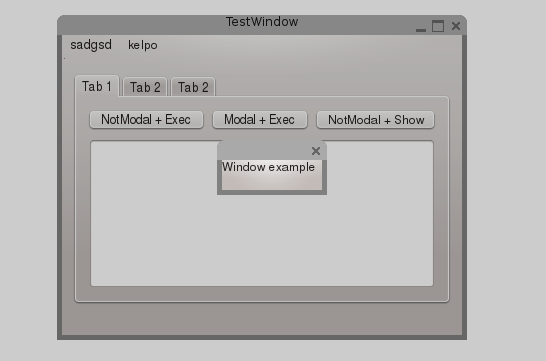
\includegraphics[width=0.7\linewidth]{img/modal}
\caption{Okno modalne -- obszar za oknem jest zacieniowany i niedostępny.}
\label{fig:modal}
\end{figure}

\begin{figure}
\centering
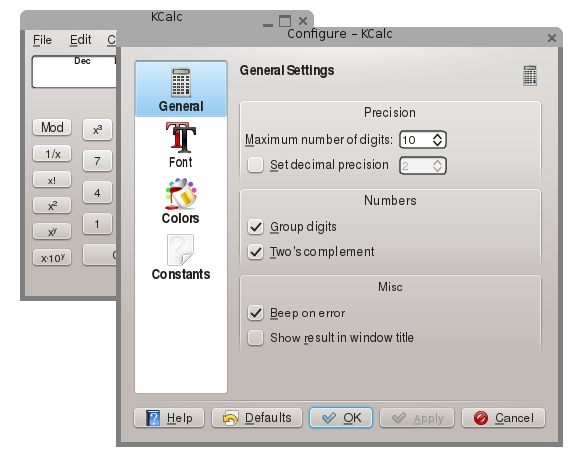
\includegraphics[width=0.7\linewidth]{img/non_modal}
\caption{Okno niemodalne -- obszar za oknem jest dostępny.}
\label{fig:non_modal}
\end{figure}


Zaimplementowana funkcjonalność maksymalizacji okna po stronie przeglądarki różni się od funkcjonalności w rzeczywistym środowisku (po stronie serwera). Maksymalizacja polega na zwiększeniu rozmiarów okna do maksymalnego dostępnu obszaru na stronie HTML.
Takie rozwiązanie wynika z możliwości uruchomienia serwera aplikacji w serwerze X11 w dowolnej rozdzielczości. Po faktycznym zmaksymalizowaniu okna na serwerze użytkownik po stronie przeglądarki widziałby okno o rozmiarze innym niż pełny dostępny obszar widoku w przeglądarce. W przypadku rozmiaru mniejszego skutkowałoby to pustym, niezagospodarowanym miejscem w oknie przeglądarki, natomiast większy rozmiar powodowałby pojawienie się suwaków przewijania (ang. scrollbar).

Funkcjonalność minimalizacji okna jest również symulowana. Okno jest chowane poprzez zmianę wartości CSS \emph{display} na \emph{none}. Dodatkowo tworzony jest element na pasku zadań, który po kliknięciu przywraca ukryte okno. Pasek zadań jest elementem strony znajdującym się na samym dole. Przykładowy pasek z jedną zminimalizowaną aplikacją przedstawia rysunek \ref{fig:taskbar}

\begin{figure}
\centering
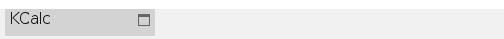
\includegraphics[width=0.7\linewidth]{img/taskbar}
\caption{Przykładowy pasek zadań z aplikacją \emph{KCalc}}
\label{fig:taskbar}
\end{figure}


\subsection{Rysowanie pojedynczego widgeta}

Widget reprezentowany jest przez element \emph{div} zawierający dwa elementy: element \emph{canvas} oraz kontener \emph{div} na widgety potomne posiadające analogiczną struktruę. Element ten ma pełni funkcję pomocniczą (jest w pełni przeźroczysty) i służy do umiejscowienia elementu w stosounku do jego rodzica za pomocą atrybutów CSS \emph{left} oraz \emph{top}. Taka implementacja relacji rodzic-dziecko widgetów na stronie zapewnia strukturę drzewiastą i łatwość zarządzania widgetami. Zmiana rodzica widgeta, który posiada zagnieżdzone dzieci nie jest problematyczna, a ze względu na format przesyłanych danych od serwera ta operacja jest bardzo często używana na etapie tworzenia okien.

Widgety z flagą \emph{Qt::Window}, czyli przede wszystkim dziedziczące z \emph{QDialog} oraz \emph{QMainWindow} są traktowane w specjalny sposób. Są opakowywane w kontener okna opisany powyżej i są elementami stojącymi najwyżej w strukturze drzewa.

\begin{figure}
\centering
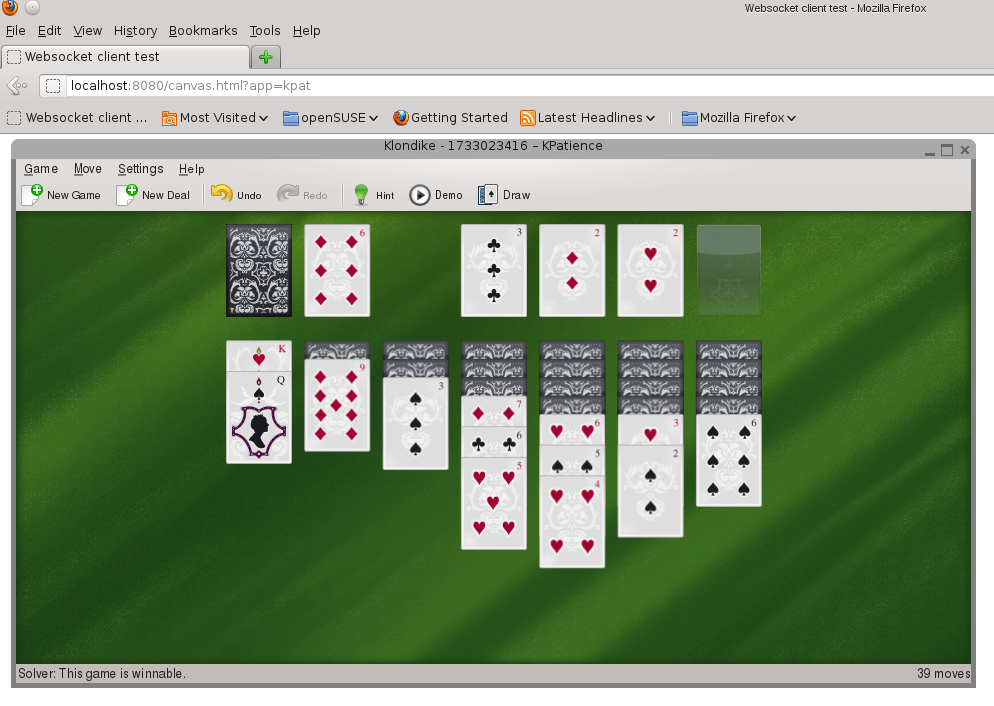
\includegraphics[width=0.7\linewidth]{img/example}
\caption{Przykład skomplikowanej aplikacji \emph{KPatience} z wieloma widgetami uruchomionej w przeglądarce \emph{Mozilla Firefox}.}
\label{fig:example}
\end{figure}


\label{sec:napotkane_problemy}
\section{Napotkane problemy}
\subsubsection{Rysowanie za pomocą zdarzeń, synchronizacja i buforowanie.}
\label{rendering_events}

Rysowanie widgetów we frameworku \emph{Qt} realizowane jest wewnątrz kolejki zdarzeń aplikacji. Zdarzenie rysowania powiadamia element interfejsu o konieczności przerysowania. Widget posiada wskaźnik do miejsca w pamięci gdzie powinien przeprowadzic operację renderowania, gdyż sam jest implementacją klasy \emph{QPaintDevice}. 

Powyższy schemat działania wymagał znalezienia sposobu na zmuszenie widgetów do rysowania za pomocą specjalnie przygotowanej implementacji klasy QPaintEngine oraz QPaintDevice. Do tego celu wykorzystana została metoda biblioteki Qt:

\begin{lstlisting}[language=C++,numbers=none]
void QWidget::render(QPainter * painter, 
                     const QPoint & targetOffset = QPoint(), 
                     const QRegion & sourceRegion = QRegion(), 
                     RenderFlags renderFlags 
                          = RenderFlags(DrawWindowBackground | 
                                        DrawChildren))
\end{lstlisting}

Umożliwia ona wskazanie obiektu \emph{QPainter} wykorzystującego mechanizm renderowania serwera, tj. reimplementacje klasy \emph{QPaintEngine} oraz \emph{QPaintDevice}. Wykorzystanie tej metody powoduje wygenerowanie kolejnego zdarzenia i umieszczenie go w kolejce aplikacji. Powodowało to problem wpadania serwera w nieskończoną pętlę i uniemożliwiało jego dalsze poprawne funkcjonowanie. 

Rozwiązaniem problemu było stworzenie własnej kolejki widgetów, które wymagają renderowania. Kolejka ta jest opróżniana w pewnych odstępach czasu nie krótszych niż 100 milisekund. Wartość ta została dobrana eksperymentalnie tak aby uzyskać efekt płynnej interakcji z aplikacją.

\subsubsection{Znikający \emph{focus} okna aplikacji.}
\label{problems_focus}

Biblioteka \emph{Qt} stanowi niejako nakładkę dla natywnego zarządcy okien systemu operacyjnego. W zwizku z tym o kolejności okien na stosie decyduje system operacyjny. \emph{Qt} podejmuje jedynie odpowiednie czynności w celu aktualizacji graficznego interfejsu aplikacji w zależności od aktualnego stanu konkretnych okien definiowanego przez system operacyjny. W sytuacji kiedy użytkownik nie prowadzi żadnej intrakcji z systemem operacyjnym a jedynie z aplikacją, mogło by się zdarzyć, że niektóre zdarzenia były by ignorowane przez aplikację. Przykładem takiej sytuacji jest wprowadzanie tekstu na klawiaturze. \emph{Qt} przesyła zdarzenia klawiatury do widgeta, który aktualnie posiada focus w oknie, które znajduje się na szczycie stosu okien w systemie operacyjnym. W momencie kiedy dwóch zdalnych użytkowników uruchomiło by aplikację na tym samym serwerze, zdarzenia jednego użytkownika były by ignorowane ponieważ tylko jedno okno jednej aplikacji może być na szczycie stosu. 

Rozwiązaniem tego problemu była reimplementacja odpowiednich metod \emph{Qt} w celu symulacji zachowania stosu okien systemu operacyjnego wewnątrz samej aplikacji. W rezultacie aplikacja działa tak jakby zawsze była aktywna, dzięki czemu framework \emph{Qt} poprawnie renderuje wszystkie elementy interfejsu użytkownika.

\subsubsection{Kody znaków klawiatury.}
\label{problems_keyboard}

\emph{Qt} dostarcza platformowo niezależny opis kodów znaków klawiatury za pomocą zdefiniowanego typu wyliczeniowego \emph{Qt::Key}\footnote{http://doc.qt.digia.com/qt/qt.html\#Key-enum}. Niestety przeglądarki nie są dobrze ustandaryzowane i ich numeracja klawiszy znacznie różni się nie tylko między samymi platformami ale również między ich wersjami. Dodatkowo przeglądarki często nie wspierają wszystkich klawiszy przez to zakres kodów znaków jest inny niż w przypadku biblioteki \emph{Qt}.

Powyższe problemy wymusiły konieczność zaimplementowania metody konwertującej po stronie klienta kody klawiszy na odpowiadające im wartości typu wyliczeniowego \emph{Qt::Key}. Kod metody znajduje się w dodatkach (\ref{lst:addons_keyboard_method})

\subsubsection{Niedopasowanie czcionek.}
\label{problems_fonts}

Wiele aplikacji wykorzystuje niestandardowe czcionki, które nie są powszechnie dostępne na większości systemach operacyjncyh. Problem jest o tyle istotny, że w przypadku braku odpowiedniej czcionki po stronie klienta tekst (np. na przyciskach lub menu podręcznym) będzie zbyt mały aby go przeczytać lub zbyt duży aby w całości zmieścić się w obszarze elementu. 

Problem ten został rozwiązany w dwojaki sposób. Po pierwsze serwer przesyła listę rodzin czcionek, które mogą zostać wykorzystane jako alternatywy. Po drugie serwer dokonuje pomiar tekstu po jego wyrenderowaniu i przesyła tą informację do klienta gdzie wynikowy tekst moze zostać dodatkowo przeskalowany w celu osiągnięcia maksymalnej zgodności.

\subsubsection{Problemy z obcinaniem (ang. clipping) w przeglądarkach.}
\label{problems_clipping}
Podczas implementacji obcinania (ang. clipping) w kliencie rozpoznano problem z implementacją tej funkcjonalności w dwóch testowanych przeglądarkach -- \emph{Mozilla Firefox} w wersji 16.0.2 oraz \emph{Google Chrome} w wersji 23.0.1271.95 m. Problem jest znany i zgłoszony\footnote{http://code.google.com/p/chromium/issues/detail?id=135559}.

\subsubsection{Synchroniczne ładowanie obrazków}

Wszystkie grafiki używane do renderowania w elementach \emph{canvas} wymagają pełnego załadowania ich do pamięci przeglądarki. Język \emph{Javascript} nie pozwala na przeprowadzenie tej operacji synchroniczne. Pełny obraz dostępny jest dopiero w asynchronicznym wywołaniu zwrotnym (ang. callback), które jest całkowicie niedeterministyczne czasowo, to znaczy nie jest określona kolejność rozpoczęcia wczytywania obrazów. Protokół komunikacji i specyfika elemntu \emph{canvas} -- pozwalająca na rysowanie tylko na wierzchu elementu -- wymusza rysowanie elementów na widgetach w odpowiedniej kolejności. Jest to sprzeczne z asynchronicznością wywołań zwrotnych, dlatego przed rozpoczęciem rysowania danego widgetu ładowane są wszystkie potrzebne obrazki. Używana jest do tego metoda \emph{delayCallback} w listingu \ref{lst:source_images_delay}. Pierwszym argumentem jest liczba obrazków do załadowania, drugim funkcja zwrotna, która zostanie wywołana po załadowaniu się wszystkich obrazów. Funkcja zwraca domknięcie, które należy wywołać w każdym wywołaniu zwrotnym załadowania obrazu (\emph{onload}).

\label{lst:source_images_delay}
\begin{lstlisting}[language=JavaScript,numbers=left,caption={Metoda łącząca wywołania wielu callbacków w jeden},label={lst:source_images_delay}]
var delayCallback = function (num, callback) {
    function finished() {
        num -= 1;
        if (num == 0 && callback) {
            callback();
        }
    }
    return finished;
};
\end{lstlisting}



\chapter{Testy aplikacji}
Natestowaliśmy się, że hoho

\section{Testy w środowisku lokalnym}
...

\section{Testy w sieci Internet}
Wszystko wyszło gitara. Jesteśmy z siebie dumni. Pozdrawiamy mamę, tatę i dudniącego Krzysztofa.


\chapter{Podsumowanie}
Temat pracy inżynierskiej został w pełni zrealizowany, a jej wynikiem jest prototyp serwera oraz webowej aplikacji klienckiej. 

Program serwera udostępnia kod strony WWW, który uruchamiany jest przez przeglądarkę. Uruchamia on również aplikację graficzną opartą o framework Qt oraz odpowiada za utworzenie połączenia między klientem a procesem aplikacji. Możliwa jest także obsługa wielu połączeń równocześnie. 
Przy pomocy techniki wstrzykiwania kodu bibliotek linkowanych dynamicznie \emph{(ang. DLL injection)} oraz wewnętrznych mechanizmów biblioteki \emph{Qt}, użycie aplikacji nie wymaga ponownej kompilacji, zarówno samego frameworka \emph{Qt}, jak i uruchamianych aplikacji użytkowych.

Aplikacja kliencka stworzona w postaci dynamicznej strony WWW pokrywa bardzo duży podzbiór funkcjonalności modułu graficznych interfejsów biblioteki \emph{Qt}. Wszelkie braki wynikają z niedoskonałości standardu HTML5, który wciąż jest mocno rozwijany.

Projekt będzie kontynuowany w następujących kierunkach:
\begin{itemize}
  \item umożliwienie współpracy z aplikacjami opartymi o najnowszą bibliotekę \emph{Qt} w wersji \emph{5.0},
  \item rozwinięcie zabezpieczeń --- autentykacja i autoryzacja klientów,
  \item stworzenie panelu administracyjnego serwera oraz nowego widoku głównego aplikacji,
  \item automatyzacja procesu instalacji,
  \item utworzenie wersji serwera dla systemów \emph{Windows} oraz \emph{Mac OS},
  \item rozwinięcie możliwości aplikacji klienckiej przy wykorzystaniu elementów technologii \emph{HTML5}, które będą dostępne w przyszłości.
\end{itemize}



%+Make Index
\printindex
%-Make Index

\end{document}